\documentclass[10pt, oneside]{article} 
\usepackage{amsmath, amsthm, amssymb, calrsfs, wasysym, verbatim, bbm, color, graphics, geometry, esint, float}


\geometry{tmargin=.75in, bmargin=.75in, lmargin=.75in, rmargin = .75in}  

\newcommand{\bbR}{\mathbb{R}}
\newcommand{\bbC}{\mathbb{C}}
\newcommand{\bbZ}{\mathbb{Z}}
\newcommand{\bbP}{\mathbb{P}}
\newcommand{\bbN}{\mathbb{N}}
\newcommand{\bbQ}{\mathbb{Q}}
\newcommand{\Cdot}{\boldsymbol{\cdot}}
\newcommand{\scA}{\mathscr{A}}
\newcommand{\curl}{\text{curl}}
\newcommand{\Ind}{\text{Ind}}
\newcommand{\Log}{\text{Log}}
\newcommand{\Vol}{\text{Vol}}


\newcommand{\sm}{\setminus}

\theoremstyle{definition}
\newtheorem{exmp}{Example}[section]
\newtheorem{thm}{Theorem}
\newtheorem{defn}{Definition}
\newtheorem{prop}{Proposition}
\newtheorem{conv}{Convention}
\newtheorem{rem}{Remark}
\newtheorem{lem}{Lemma}
\newtheorem{cor}{Corollary}
% Copyright 2021 Paolo Adajar (padajar.com, paoloadajar@mit.edu)
% 
% Permission is hereby granted, free of charge, to any person obtaining a copy of this software and associated documentation files (the "Software"), to deal in the Software without restriction, including without limitation the rights to use, copy, modify, merge, publish, distribute, sublicense, and/or sell copies of the Software, and to permit persons to whom the Software is furnished to do so, subject to the following conditions:
%
% The above copyright notice and this permission notice shall be included in all copies or substantial portions of the Software.
% 
% THE SOFTWARE IS PROVIDED "AS IS", WITHOUT WARRANTY OF ANY KIND, EXPRESS OR IMPLIED, INCLUDING BUT NOT LIMITED TO THE WARRANTIES OF MERCHANTABILITY, FITNESS FOR A PARTICULAR PURPOSE AND NONINFRINGEMENT. IN NO EVENT SHALL THE AUTHORS OR COPYRIGHT HOLDERS BE LIABLE FOR ANY CLAIM, DAMAGES OR OTHER LIABILITY, WHETHER IN AN ACTION OF CONTRACT, TORT OR OTHERWISE, ARISING FROM, OUT OF OR IN CONNECTION WITH THE SOFTWARE OR THE USE OR OTHER DEALINGS IN THE SOFTWARE.

\usepackage{fullpage}
\usepackage{enumitem}
\usepackage{amsfonts, amssymb, amsmath,amsthm}
\usepackage{mathtools}
\usepackage[pdftex, pdfauthor={\name}, pdftitle={\classnum~\assignment}]{hyperref}
\usepackage[dvipsnames]{xcolor}
\usepackage{bbm}
\usepackage{graphicx}
\usepackage{mathrsfs}
\usepackage{pdfpages}
\usepackage{tabularx}
\usepackage{pdflscape}
\usepackage{makecell}
\usepackage{booktabs}
\usepackage{natbib}
\usepackage{caption}
\usepackage{subcaption}
\usepackage{physics}
\usepackage[many]{tcolorbox}
\usepackage{version}
\usepackage{ifthen}
\usepackage{cancel}
\usepackage{listings}
\usepackage{courier}

\usepackage{tikz}
\usepackage{istgame}

\hypersetup{
	colorlinks=true,
	linkcolor=blue,
	filecolor=magenta,
	urlcolor=blue,
}

\setlength{\parindent}{0mm}
\setlength{\parskip}{2mm}

\setlist[enumerate]{label=({\alph*})}
\setlist[enumerate, 2]{label=({\roman*})}

\allowdisplaybreaks[1]

\newcommand{\psetheader}{
	\ifthenelse{\isundefined{\collaborators}}{
		\begin{center}
			{\setlength{\parindent}{0cm} \setlength{\parskip}{0mm}
				
				{\textbf{\classnum~\semester:~\assignment} \hfill \name}
				
				\subject \hfill \href{mailto:\email}{\tt \email}
				
				Instructor(s):~\instructors \hfill Due Date:~\duedate	
				
				\hrulefill}
		\end{center}
	}{
		\begin{center}
			{\setlength{\parindent}{0cm} \setlength{\parskip}{0mm}
				
				{\textbf{\classnum~\semester:~\assignment} \hfill \name\footnote{Collaborator(s): \collaborators}}
				
				\subject \hfill \href{mailto:\email}{\tt \email}
				
				Instructor(s):~\instructors \hfill Due Date:~\duedate	
				
				\hrulefill}
		\end{center}
	}
}

\renewcommand{\thepage}{\classnum~\assignment \hfill \arabic{page}}

\makeatletter
\def\points{\@ifnextchar[{\@with}{\@without}}
\def\@with[#1]#2{{\ifthenelse{\equal{#2}{1}}{{[1 point, #1]}}{{[#2 points, #1]}}}}
\def\@without#1{\ifthenelse{\equal{#1}{1}}{{[1 point]}}{{[#1 points]}}}
\makeatother

\newtheoremstyle{theorem-custom}%
{}{}%
{}{}%
{\itshape}{.}%
{ }%
{\thmname{#1}\thmnumber{ #2}\thmnote{ (#3)}}

\theoremstyle{theorem-custom}

\newtheorem{theorem}{Theorem}
\newtheorem{lemma}[theorem]{Lemma}
\newtheorem{example}[theorem]{Example}

\newenvironment{problem}[1]{\color{black} #1}{}

\newenvironment{solution}{%
	\leavevmode\begin{tcolorbox}[breakable, colback=green!5!white,colframe=green!75!black, enhanced jigsaw] \proof[\scshape Solution:] \setlength{\parskip}{2mm}%
	}{\renewcommand{\qedsymbol}{$\blacksquare$} \endproof \end{tcolorbox}}

\newenvironment{reflection}{\begin{tcolorbox}[breakable, colback=black!8!white,colframe=black!60!white, enhanced jigsaw, parbox = false]\textsc{Reflections:}}{\end{tcolorbox}}

\newcommand{\qedh}{\renewcommand{\qedsymbol}{$\blacksquare$}\qedhere}

\definecolor{mygreen}{rgb}{0,0.6,0}
\definecolor{mygray}{rgb}{0.5,0.5,0.5}
\definecolor{mymauve}{rgb}{0.58,0,0.82}

% from https://github.com/satejsoman/stata-lstlisting
% language definition
\lstdefinelanguage{Stata}{
	% System commands
	morekeywords=[1]{regress, reg, summarize, sum, display, di, generate, gen, bysort, use, import, delimited, predict, quietly, probit, margins, test},
	% Reserved words
	morekeywords=[2]{aggregate, array, boolean, break, byte, case, catch, class, colvector, complex, const, continue, default, delegate, delete, do, double, else, eltypedef, end, enum, explicit, export, external, float, for, friend, function, global, goto, if, inline, int, local, long, mata, matrix, namespace, new, numeric, NULL, operator, orgtypedef, pointer, polymorphic, pragma, private, protected, public, quad, real, return, rowvector, scalar, short, signed, static, strL, string, struct, super, switch, template, this, throw, transmorphic, try, typedef, typename, union, unsigned, using, vector, version, virtual, void, volatile, while,},
	% Keywords
	morekeywords=[3]{forvalues, foreach, set},
	% Date and time functions
	morekeywords=[4]{bofd, Cdhms, Chms, Clock, clock, Cmdyhms, Cofc, cofC, Cofd, cofd, daily, date, day, dhms, dofb, dofC, dofc, dofh, dofm, dofq, dofw, dofy, dow, doy, halfyear, halfyearly, hh, hhC, hms, hofd, hours, mdy, mdyhms, minutes, mm, mmC, mofd, month, monthly, msofhours, msofminutes, msofseconds, qofd, quarter, quarterly, seconds, ss, ssC, tC, tc, td, th, tm, tq, tw, week, weekly, wofd, year, yearly, yh, ym, yofd, yq, yw,},
	% Mathematical functions
	morekeywords=[5]{abs, ceil, cloglog, comb, digamma, exp, expm1, floor, int, invcloglog, invlogit, ln, ln1m, ln, ln1p, ln, lnfactorial, lngamma, log, log10, log1m, log1p, logit, max, min, mod, reldif, round, sign, sqrt, sum, trigamma, trunc,},
	% Matrix functions
	morekeywords=[6]{cholesky, coleqnumb, colnfreeparms, colnumb, colsof, corr, det, diag, diag0cnt, el, get, hadamard, I, inv, invsym, issymmetric, J, matmissing, matuniform, mreldif, nullmat, roweqnumb, rownfreeparms, rownumb, rowsof, sweep, trace, vec, vecdiag, },
	% Programming functions
	morekeywords=[7]{autocode, byteorder, c, _caller, chop, abs, clip, cond, e, fileexists, fileread, filereaderror, filewrite, float, fmtwidth, has_eprop, inlist, inrange, irecode, matrix, maxbyte, maxdouble, maxfloat, maxint, maxlong, mi, minbyte, mindouble, minfloat, minint, minlong, missing, r, recode, replay, return, s, scalar, smallestdouble,},
	% Random-number functions
	morekeywords=[8]{rbeta, rbinomial, rcauchy, rchi2, rexponential, rgamma, rhypergeometric, rigaussian, rlaplace, rlogistic, rnbinomial, rnormal, rpoisson, rt, runiform, runiformint, rweibull, rweibullph,},
	% Selecting time-span functions
	morekeywords=[9]{tin, twithin,},
	% Statistical functions
	morekeywords=[10]{betaden, binomial, binomialp, binomialtail, binormal, cauchy, cauchyden, cauchytail, chi2, chi2den, chi2tail, dgammapda, dgammapdada, dgammapdadx, dgammapdx, dgammapdxdx, dunnettprob, exponential, exponentialden, exponentialtail, F, Fden, Ftail, gammaden, gammap, gammaptail, hypergeometric, hypergeometricp, ibeta, ibetatail, igaussian, igaussianden, igaussiantail, invbinomial, invbinomialtail, invcauchy, invcauchytail, invchi2, invchi2tail, invdunnettprob, invexponential, invexponentialtail, invF, invFtail, invgammap, invgammaptail, invibeta, invibetatail, invigaussian, invigaussiantail, invlaplace, invlaplacetail, invlogistic, invlogistictail, invnbinomial, invnbinomialtail, invnchi2, invnF, invnFtail, invnibeta, invnormal, invnt, invnttail, invpoisson, invpoissontail, invt, invttail, invtukeyprob, invweibull, invweibullph, invweibullphtail, invweibulltail, laplace, laplaceden, laplacetail, lncauchyden, lnigammaden, lnigaussianden, lniwishartden, lnlaplaceden, lnmvnormalden, lnnormal, lnnormalden, lnwishartden, logistic, logisticden, logistictail, nbetaden, nbinomial, nbinomialp, nbinomialtail, nchi2, nchi2den, nchi2tail, nF, nFden, nFtail, nibeta, normal, normalden, npnchi2, npnF, npnt, nt, ntden, nttail, poisson, poissonp, poissontail, t, tden, ttail, tukeyprob, weibull, weibullden, weibullph, weibullphden, weibullphtail, weibulltail,},
	% String functions 
	morekeywords=[11]{abbrev, char, collatorlocale, collatorversion, indexnot, plural, plural, real, regexm, regexr, regexs, soundex, soundex_nara, strcat, strdup, string, strofreal, string, strofreal, stritrim, strlen, strlower, strltrim, strmatch, strofreal, strofreal, strpos, strproper, strreverse, strrpos, strrtrim, strtoname, strtrim, strupper, subinstr, subinword, substr, tobytes, uchar, udstrlen, udsubstr, uisdigit, uisletter, ustrcompare, ustrcompareex, ustrfix, ustrfrom, ustrinvalidcnt, ustrleft, ustrlen, ustrlower, ustrltrim, ustrnormalize, ustrpos, ustrregexm, ustrregexra, ustrregexrf, ustrregexs, ustrreverse, ustrright, ustrrpos, ustrrtrim, ustrsortkey, ustrsortkeyex, ustrtitle, ustrto, ustrtohex, ustrtoname, ustrtrim, ustrunescape, ustrupper, ustrword, ustrwordcount, usubinstr, usubstr, word, wordbreaklocale, worcount,},
	% Trig functions
	morekeywords=[12]{acos, acosh, asin, asinh, atan, atanh, cos, cosh, sin, sinh, tan, tanh,},
	morecomment=[l]{//},
	% morecomment=[l]{*},  // `*` maybe used as multiply operator. So use `//` as line comment.
	morecomment=[s]{/*}{*/},
	% The following is used by macros, like `lags'.
	morestring=[b]{`}{'},
	% morestring=[d]{'},
	morestring=[b]",
	morestring=[d]",
	% morestring=[d]{\\`},
	% morestring=[b]{'},
	sensitive=true,
}

\lstset{ 
	backgroundcolor=\color{white},   % choose the background color; you must add \usepackage{color} or \usepackage{xcolor}; should come as last argument
	basicstyle=\footnotesize\ttfamily,        % the size of the fonts that are used for the code
	breakatwhitespace=false,         % sets if automatic breaks should only happen at whitespace
	breaklines=true,                 % sets automatic line breaking
	captionpos=b,                    % sets the caption-position to bottom
	commentstyle=\color{mygreen},    % comment style
	deletekeywords={...},            % if you want to delete keywords from the given language
	escapeinside={\%*}{*)},          % if you want to add LaTeX within your code
	extendedchars=true,              % lets you use non-ASCII characters; for 8-bits encodings only, does not work with UTF-8
	firstnumber=0,                % start line enumeration with line 1000
	frame=single,	                   % adds a frame around the code
	keepspaces=true,                 % keeps spaces in text, useful for keeping indentation of code (possibly needs columns=flexible)
	keywordstyle=\color{blue},       % keyword style
	language=Octave,                 % the language of the code
	morekeywords={*,...},            % if you want to add more keywords to the set
	numbers=left,                    % where to put the line-numbers; possible values are (none, left, right)
	numbersep=5pt,                   % how far the line-numbers are from the code
	numberstyle=\tiny\color{mygray}, % the style that is used for the line-numbers
	rulecolor=\color{black},         % if not set, the frame-color may be changed on line-breaks within not-black text (e.g. comments (green here))
	showspaces=false,                % show spaces everywhere adding particular underscores; it overrides 'showstringspaces'
	showstringspaces=false,          % underline spaces within strings only
	showtabs=false,                  % show tabs within strings adding particular underscores
	stepnumber=2,                    % the step between two line-numbers. If it's 1, each line will be numbered
	stringstyle=\color{mymauve},     % string literal style
	tabsize=2,	                   % sets default tabsize to 2 spaces
%	title=\lstname,                   % show the filename of files included with \lstinputlisting; also try caption instead of title
	xleftmargin=0.25cm
}



\title{UChicago Real Analysis III Notes: 20510}
\author{Notes by Agustín Esteva, Lectures by Donald Stull, Books by Rudin, Stein and Shakarchi}
\date{Academic Year 2024-2025}

\begin{document}

\maketitle
\tableofcontents

\vspace{.25in}


\newpage
\section{Lectures}

\subsection{Monday, Mar 24: Motivation for the Lebesgue Measure}
\begin{defn}
    A family of sets $\mathcal{A}$ is called a \textbf{ring} if it is closed under finite unions and under set complements. 
\end{defn}
\begin{defn}
    A ring is called a \textbf{$\sigma-$ring} if it is closed under countable unions.
\end{defn}
\begin{rem}
    I will most often refer to $\sigma-$rings as $\sigma-$algebra. The only difference if $\mathcal{F}$ is a $\sigma-$algebra, then if $A \in \cal F,$ then $A^c \in \cal F.$ Meanwhile, if $A\in \cal A,$ then $A^c$ might not necessarily be in the ring. Instead, if $B \in \cal A,$ then $B\sm A \in \cal A.$  
\end{rem}
Using DeMorgan's Law, a $\cal F$ is closed under countable intersections as well. 
\begin{defn}
    A \textbf{set function} $\phi$ on an algebra $\cal F$ satisfies that for all $A \in \cal F,$ $\phi(A) \in \bbR \cup \{\pm \infty\}$ (but not both at the same time).
\end{defn}
\begin{defn}
A set function $\phi$ is \textbf{additive} if for all $A,B$ disjoint, we have that 
\[\phi(A\sqcup B) = \phi(A) + \phi(B).\]
\end{defn}
\begin{defn}
    We say that $\phi$ is \textbf{countably additive} if for any $A_1, A_2, \dots$ mutually disjoint, we have that 
    \[\phi\left(\bigsqcup_{n=1}^\infty A_i\right) = \sum_{n=1}^\infty \phi(A_i)\]
\end{defn}
\begin{rem}
    Let $\phi$ be an additive set function on $\cal F$. Then 
    \begin{enumerate}
        \item $\phi(\emptyset) = 0.$ Let $A\in \cal F$ with $\phi(A) < \infty.$ Then $A = A \sqcup \emptyset$ and so $\phi(A) = \phi(A)+ \phi(\emptyset).$
        \item Let $N < \infty,$ then for $A_1, \dots, A_N$ mutually disjoint, 
        \[\phi\left(\bigsqcup_{n=1}^N A_i\right) = \phi\left(A_1 \sqcup \bigsqcup_{n=2}^N A_i\right) = \phi(A_1) + \phi\left(\bigsqcup_{n=2}^N A_i\right) = \cdots = \sum_{n=1}^N \phi(A_i).\]
        \item We have that for any $A,B \in \cal F,$ 
        \[\phi(A\cup B) + \phi(A\cap B) =  \phi(A)+ \phi(B)\]
        \item If $\phi$ is positive real valued, then if $A \subset B,$ then 
        \[\phi(A) \leq \phi(B).\] Notice that 
        \[\phi(B) = \phi(A \sqcup (B\sm A)) = \phi(A) + \phi(B\sm A) \geq \phi(A).\]
        \item If $A\subseteq B$ and $\phi(B) < \infty,$ then 
        \[\phi(B\sm A) = \phi(B) - \phi(A).\]
    \end{enumerate}
\end{rem}

\begin{thm}
    Let $\phi$ be a countably additive set function on $\cal F.$ Suppose $(A_n) \in \cal F$ such that $A_1 \subseteq A_2 \subseteq \cdots $ and 
    \[\bigcup_{n=1}^\infty A_i = A.\] Then $\phi(A_n) \to \phi(A).$
\end{thm}
\begin{proof}
    Define 
    \[B_1:= A_1, \quad B_2 := A_2 \sm A_1, \quad B_3:= A_3 \sm A_2, \cdots \] Then $(B_n)$ is a collection of disjoint sets such that $\bigsqcup_{n=1}^\infty B_i = A.$ Then since $\phi$ is countably additive, we have that
    \[\phi(A_n) = \phi(\bigsqcup_{i=1}^n B_i) = \sum_{i=1}^n \phi(B_i)\to \sum_{i=1}^\infty\phi(B_i) = \phi(\bigsqcup_{i=1}^\infty B_i)= \phi(A).\]
\end{proof}

\begin{defn}
    An \textbf{interval} $I = \{a_i, b_i\}_{i=1}^n \subseteq \bbR^n$ is a set of points $x = (x_1, \dots, x_n)$ such 
    \[a_i \leq x_i \leq b_i,\] where the $\leq$ can be replaced with $<.$
\end{defn}

\begin{defn}
    We say that $A$ is \textbf{elementary} if $A$ is a union of finitely many intervals. 
\end{defn}

\begin{rem}
    We call the set of elementary sets $\cal E.$
\end{rem}
\begin{defn}
    Suppose $I$ is an interval of $\bbR^n.$ Then the \textbf{volume} of $I$ is 
    \[\Vol(I) = \prod_{i=1}^n (b_i - a_i).\]
\end{defn}
\begin{rem}
    Let $A \in \cal E.$ Then $A = \bigcup_{i=1}^n I_i.$ Then 
    \[\Vol(A) = \sum_{i=1}^n \Vol(I_i)\]
\end{rem}

\newpage
\subsection{Wednesday, Mar 26: The Lebesgue Outer Measure}
\begin{rem}
    \begin{enumerate}
        \item $\cal E$ is a ring, but not a $\sigma-$ring.
        \item If $A\in \cal E,$ then $A$ can be decomposed into a finite union of disjoint intervals.
        \item If $A\in \cal E,$ then $\Vol(A)$ is well defined. 
    \end{enumerate}
\end{rem}

\begin{defn}
    A non-negative set function on $\cal E$ is called \textbf{regular} if for all $A\in \cal E,$ for all $\epsilon>0,$ there exists  open $O  \in \cal E$ and closed $F \in \cal E$ such that $F\subseteq A \subseteq O$ and 
    \[\phi(G) \leq \phi(A) + \epsilon, \quad \phi(A) \leq \phi(F)  + \epsilon.\]
\end{defn}
Note that $\Vol$ is regular. 
\begin{defn}
    The \textbf{Lebesgue Outer Measure} of $E\subseteq \bbR^n$ is defined by
    \[m^*(E) = \inf\left(\sum_{n=1}^\infty \Vol(A_i)\right),\] where the infemum is taken over all the countable open covers of $E.$ 
\end{defn}

\begin{rem}
Let $E\in \bbR^n.$ Then
    \begin{enumerate}
        \item $m^*(E)$ is well defined.
        \item If $E_1\subseteq E_2 \subseteq\bbR^n.$ Then 
        \[m^*(E_1) \leq m^*(E_2).\]
        \item The outer measure is non-negative.
    \end{enumerate}
\end{rem}

\begin{thm}
    If $A\in \cal E,$ then $\Vol(A) = m^*(A).$ Moreover, if $E = \bigcup_{i=1}^\infty E_i,$ then $m^*(E) \leq \sum_{i=1}^\infty m^*(E_i)$
\end{thm}

\begin{proof}
    Let $\epsilon>0.$ Since $\Vol$ is regular, then there exists some open $O \supseteq A$ such that $\Vol(O) \leq \Vol(A) + \epsilon.$ Since $O$ is an open cover, we have that $m^*(A) \leq \Vol(O) \leq \Vol(A) + \epsilon.$ Thus, $m^*(A) \leq \Vol(A) + \epsilon.$ Let $F \subseteq A$ closed such that $\Vol(A) \leq \Vol(F) + \frac{\epsilon}{2}.$ Then since $F$ is closed and bounded in $\bbR^n,$ it is compact. Let $\{A_n\}_{n=1}^\infty$ be an open cover of $A$ such that 
    \[\sum_{n=1}^\infty \Vol(A_i) \leq   m^*(A) + \frac{\epsilon}{2}\]
    Then there exists $\{A_n\}_{n=1}^N$ finite open cover of $F$ by compactness. By the finite sub-additivity of $F,$ we have that 
    \[\Vol(A) \leq \Vol(F) + \frac{\epsilon}{2} \leq \sum_{n=1}^N \Vol(A_n) + \frac{\epsilon}{2} \leq \sum_{n=1}^\infty \Vol(A_n) + \frac{\epsilon}{2} \leq m^*(A) + \epsilon.\] Thus, $\Vol(A) \leq m^*(A).$

    Suppose $m^*(E_n) < \infty$ for all $n.$ Let $\epsilon>0.$ For each $n,$ there exists a countable open cover such that 
    \[\sum_{i=1}^\infty \Vol(A_i^{(n)}) \leq m^*(E_n) + \frac{\epsilon}{2^n}.\] Since $E\subseteq \bigcup_{n=1}^\infty \bigcup_{i=1}^\infty A_i^{(n)},$ then 
    \[m^*(E) \leq \sum_{n=1}^\infty \sum_{i=1}^\infty \Vol(A_i^{(n)}) \leq \sum_{n=1}^\infty m^*(E_n) + \frac{\epsilon}{2^n} \leq \sum_{n=1}^\infty m^*(E_n)  + \epsilon\]
\end{proof}

\newpage
\subsection{Friday, Mar 28: The Lebesgue Measure}
\begin{defn}
    Let $A, B \subseteq \bbR^n.$ The \textbf{symmetric difference} of $A$ and $B$ is 
    \[A\triangle B = (A\sm B) \cup (B\sm A)\]
\end{defn}
\begin{defn}
    The \textbf{distance} between $A$ and $B$ is defined as
    \[d(A,B) = m^*(A\triangle B).\]
\end{defn}
\begin{defn}
    Let $(A_n) \in \bbR^n.$ We say that $A_n$  \textbf{converges in (outer) measure} if $d(A_n, A) \to 0.$
\end{defn}
\begin{defn}
    If there exists a sequence $(A_n) \in \cal E$ such that $A_n \to A,$ then $A$ is \textbf{finitely-measurable}. We say that $A \in \mathcal{M}_F(m).$
\end{defn}
\begin{defn}
    We say that $E \in \mathcal{M}(m)$ if 
    \[E = \bigcup_{n=1}^\infty A_n,\] where each $A_n \in \mathcal{M}_F(m).$
\end{defn}
\begin{thm}
    (Caratheodory) $\cal M$ is a $\sigma-$family, and $m^*$ is countably additive on $\cal M.$
\end{thm}
\begin{defn}
    The \textbf{Lebesgue Measure} is the set function 
    \[m: \mathcal{M}(m) \to [0, \infty], \quad m(A) = m^*(A).\]
\end{defn}
\begin{rem}
    As a small review we recap our set-functions so far:
    \begin{table}[H]
        \centering
        \begin{tabular}{c|cl}
             Set Function&   Domain&Properties\\
             $\Vol$& 
         $\cal E$&Non-negative, Finitely Additive, Regular\\
 $m^*$& $\bbR^n$&Non-negative, Countably-sub-additive, $m|_{\cal E} = \Vol$\\
 m& $\cal M$&Non-negative, Countably-additive, $m|_{\cal M} = m^*$\\\end{tabular}
        \caption{Set Functions}

    \end{table}
\end{rem}
\begin{exmp}
\begin{enumerate}
    \item If $A \in \cal E,$ then $ A \in \cal M.$ 
    \item Since $\bbR^d = \bigcup_{n=1}^\infty [-n, n]^d,$ then $\bbR^d \in \cal M.$
    \item If $A \in \cal M,$ then $A^c \in \cal M$.
    \item For all $x\in \bbR^n,$ $x\in \cal M.$ This is because
    \[x = \bigcap_{n=1}^\infty (x- \frac{1}{n}, x + \frac{1}{n}).\] Moreover, $m(\{x\}) = 0.$ 
    \item $m(\bbQ) = 0.$
\end{enumerate}
\end{exmp}

\newpage
\subsection{Monday, Mar 31: Measurable Functions}
\begin{defn}
    We say that $f: \bbR^n \to \bbR$ is \textbf{(Lebesgue) measurable} if, for every $a\in \bbR^n,$ $\{x \in \bbR^n \mid f(x) >a\}$ is measurable.
\end{defn}
\begin{rem}
    If $f$ is continuous, then $f^{-1}\big((a, \infty)\big)$ is open, and thus measurable. Then $f$ is measurable.
\end{rem}
\begin{prop}
    Equivalently, $f$ is measurable if the following are measurable:
    \begin{itemize}
        \item $\{x \in \bbR^n \mid f(x) > a\}$ 
        \item $\{x \in \bbR^n \mid f(x) \geq a\}$ 
        \item $\{x \in \bbR^n \mid f(x) < a\}$ 
        \item $\{x \in \bbR^n \mid f(x) \leq a\}$ 
    \end{itemize}
\end{prop}
\begin{proof}
    Suppose $f$ is measurable. We can write 
    \[\{x \in \bbR^n \mid f(x) \geq a\} = \bigcap_{n=1}^\infty \{x \in \bbR^n \mid f(x) > a + \frac{1}{n}\}.\] 
    \[\{x \in \bbR^n \mid f(x) \leq a\} = \{x \in \bbR^n \mid f(x) > a\}^c\]
    \[\{x \in \bbR^n \mid f(x) < a\} = \{x \in \bbR^n \mid f(x) \geq a\}^c.\] By Caratheodory's theorem (Theorem 3), we are done. 
\end{proof}

\begin{thm}
    Suppose $f$ is measurable. Then $|f|$ is measurable.
\end{thm}
\begin{proof}
    Let $a\in \bbR^n.$ Then we can write
    \[\{x \in \bbR^n \mid |f(x)| < a\} = \{x \in \bbR^n \mid -a<f(x) < a\} = \{x \in \bbR^n \mid f(x) < a\} \cap \{x \in \bbR^n \mid f(x) >- a\}.\]
\end{proof}
\begin{thm}
    Suppose $(f_n)$ are measurable and $g = \sup f_n$ and $h = \limsup f_n.$ Then $g$ and $h$ are measurable.
\end{thm}
\begin{proof}
    Let $a\in \bbR^n.$ Then 
    \[\{x \in \bbR^n \mid g(x) > a\} = \bigcup_{n=1}^\infty \{x \in \bbR^n \mid f_n(x) >a\},\] and 
    \[\{x \in \bbR^n \mid h(x) > a\} = \bigcap_{n=1}^\infty\bigcup_{n=m}^\infty \{x \in \bbR^n \mid f_m(x) >a\}.\]
\end{proof}

\begin{cor}
\begin{enumerate}
    \item If $f,g$ are measurable, then so are $\max\{f,g\}$ and $\min\{f,g\}.$
    \item Suppose $f$ is measurable. We can write $f = f^+ - f^-,$ where $f^+ = \max\{f,0\}$ and $f^- = -\min\{f,0\}.$ Both $f^+$ and $f^-$ are measurable.
\end{enumerate}
\end{cor}

\begin{thm}
    Suppose $f,g: \bbR^n t\o \bbR$ are measurable. If $F: \bbR^2 \to \bbR$ is continuous, then $h(x) = F(f(x), g(x)).$ Then $h$ is measurable. 
\end{thm}
Thus, $f + g,$ $fg,$ and all the rest are measurable if the components are measurable.

\begin{defn}
    A function $\varphi: \bbR^n \to \bbR$ is a \textbf{simple function} if $R(\varphi) < \infty.$
\end{defn}
\begin{rem}
    Equivalently, if $\varphi$ is simple, then 
    \[\varphi = \sum_{k=1}^n c_k \chi_{E_k},\] where $R(\varphi)= \{c_1, \dots, c_n\}$ and $E_k  = \{x \in \bbR^n \mid \varphi(x)  = c_k\}.$
\end{rem}
Note that $E$ is measurable iff $\chi_E$ is measurable.
\begin{cor}
    Suppose $\vaprhi$ is a simple function. Then $\varphi$ is measurable if and only if each $E_k$ is measurable
\end{cor}


\newpage
\subsection{Wednesday, Apr 2: The Lebesgue Integral}
\begin{thm}
    Suppose $f: \bbR^n \to \bbR.$ There exists a sequence of $(\varphi_n)$ simple functions such that $\varphi_n \to f$ pointwise. Moreover, if $f\geq 0,$ then one can choose the sequence such that $0\leq \varphi_n \uparrow f.$ If $f$ is measurable, one can choose the $\varphi_n$ to be measurable.
\end{thm}
The proof can be found in the second PSET.
\begin{defn}
    Suppose $\varphi$ is a simple non-negative measurable function. Let $E\in \cal M.$ We define the \textbf{integral of a simple function} to be 
    \[I_E(\varphi) = \sum_{k=1}^n c_k m(E_k \cap E).\]
\end{defn}
\begin{defn}
    Suppose $f\geq 0$ is measurable. If $E\in \cal M,$ the define the \textbf{Lebesgue Integral} to be 
    \[\int_E f \, dm = \sup_{0 \leq\varphi \leq f, \; \varphi \text{ simple}} I_E(\varphi).\]
\end{defn}

\begin{defn}
    Suppose $f$ is measurable. We define the \textbf{Lebesgue integral of $f$} over $E \in \cal E$ to be
    \[\int_E f \, dm = \int_E f^+ \, dm -\int_E f^-\, dm.\] If either is finite, then we write that $f\in \cal L$ and say that $f$ is \textbf{Lebesgue integrable}.
\end{defn}
\begin{rem}
    \begin{itemize}
        \item The Lebesgue integral is well defined.
        \item The Lebesgue integral can be infinity.
        \item If $\varphi$ is non-negative and simple and measurable, then $\int_E \varphi = I_E(\varphi).$
    \end{itemize}
\end{rem}


\newpage
\subsection{Friday, Apr 4: Properties of the Lebesgue Integral}
\begin{rem}
Let $f$ be measurable.
\begin{enumerate}
    \item If $a\leq f(x) \leq b$ for all $x\in E \in \cal M,$ then 
    \[a \,m(E) \leq \int_E f\, dm \leq b\,m(E).\]
    \item Suppose $f$ is bounded and $E \in \cal M$ with $m(E) < \infty.$ Then $f\in \mathcal L(E).$
    \item If $f,g \in \mathcal L(E)$ and $f \leq g$ on $E,$ then 
    \[\int_E f\, dm \leq \int_E g\,dm\]
    \item If $f \in \mathcal L(E)$ and $c\in \bbR^n,$ then $cf \in \mathcal{L}(E)$ and 
    \[\int_E c f\,dm = c\int_E f \, dm.\]
    \item If $m(E) = 0,$ then 
    \[\int_E f\, dm = 0.\]
    \item If $f\in \mathcal L(A)$ and $A \in \cal M$ and $E\subseteq A,$ then $f\in \mathcal L(E).$
    \item If $f\in \mathcal{R}([a,b]),$ then $f \in \mathcal{L}([a,b])$ and the Riemann integrals and Lebesgue integrals are equivalent. 
\end{enumerate}
\end{rem}
\begin{thm}
    Suppose $f\geq 0$ is measurable. For all $A\in \cal M,$ define the set function 
    \[\phi(A) = \int_A f\, dm.\] Then $\phi$ is countably additive.
\end{thm}
\begin{proof}
Suppose $(A_n) \in \cal M.$
\begin{itemize}
    \item Suppose $f$ is a characteristic function. That is, $f = \chi_E$ for some $E\in \cal M.$ Then 
    \[\phi(\bigsqcup_{n=1}^\infty A_n) = \int_{\bigsqcup_{n=1}^\infty A_n} f = m(E \cap \bigsqcup_{n=1}^\infty A_n) = m(\bigsqcup_{n=1}^\infty E \cap A_n) = \sum_{n=1}^\infty m(E \cap A_n) = \sum_{n=1}^\infty \phi(A_n)\]
    \item Suppose $f$ is simple function. That is, $f = \sum_{k=1}^N c_k E_k.$ Then 
    \begin{align*}
    \phi(\bigsqcup_{n=1}^\infty A_n) &= \int_{\bigsqcup A_n}f \, dm\\ &= \int_{\bigsqcup A_n} \sum_{k=1}^N c_k \chi_{E_k}\, dm\\ &= \sum_{k=1}^N c_k \phi(\bigsqcup_{n=1}^\infty \chi_{E_k})\\ &= \sum_{k=1}^N c_k \sum_{n=1}^\infty \phi(\chi_{E_k})\\ &= \sum_{n=1}^\infty \sum_{k=1}^N c_k m(E_k \cap A_n)\\ &= \sum_{n=1}^\infty\int_{A_n} f\\ &= \sum_{n=1}^\infty \phi(A_n)    
    \end{align*}
    \item Suppose $f \geq 0.$ Let $0\leq\varphi \leq f$ be measurable. Then we know that 
    \[\int_{\bigsqcup A_n} \varphi \leq \sum_{n=1}^\infty \int_{A_n} \varphi\, dm \leq \sum_{n=1}^\infty \int_{A_n} f \, dm = \sum_{n=1}^\infty\phi(A_n).\]
    Let $\epsilon>0.$ By definition, there exists a simple function $\varphi$ such that 
    \[\int_{A_n} \varphi \geq \int_{A_n} f - \frac{\epsilon}{2^n}.\] Then 
    \[\phi(\bigsqcup_{n=1}^k A_n) \geq \int_{\bigsqcup_{n=1}^k A_n}\varphi \, dm \geq \sum_{n=1}^k \phi(A_n) - \frac{\epsilon}{2^n} \to \sum_{n=1}^\infty \phi(A_n) - \epsilon.\]
\end{itemize}
\end{proof}

\begin{cor}
    Suppose $A, B \in \cal M$ with $B \subseteq A$ such that $m(A\sm B) = 0.$ Then for all $f\in \mathcal{L}(A),$ we have that 
    \[\int_A f \, dm = \int_B f\, dm\]
\end{cor}
\begin{proof}
    Write $A = B \sqcup A\sm B$ and conclude using the previous theorem and remark 11.
\end{proof}


\newpage
\subsection{Monday, Apr 7: Lebesgue's Monotone Convergence Theorem}
\begin{thm}
    Suppose $f \in \mathcal{L}(E).$ Then $|f| \in \mathcal{L}(E)$ and 
    \[\left|\int_E f\, dm\right| \leq \int_E |f|\, dm\]
\end{thm}

\begin{proof}
   Let \[A:= \{x \in E \mid f(x) \geq 0\}, \quad B:= \{x \in E \mid f(x) < 0\}.\] Then $E = A\sqcup B$ and so 
   \[\int_E |f|\, dm = \int_A |f|\, dm + \int_B |f|\, dm = \int_A f^+ \, dm + \int_B f^- \, dm < \infty.\] Thus, $|f| \in \mathcal{L}(E).$ Since $f\leq |f|$ and $-f \leq |f|,$ we have that 
   \[\int_E f \, dm \leq \int_E |f|\, dm, \quad -\int_E f \, dm \leq \int_E |f|\, dm.\]
\end{proof}

\begin{thm}
    (Monotone Convergence Theorem) Suppose $f_n$ is a sequence of non-negative measurable functions with $f_1(x) \leq f_2(x) \leq \cdots $ for al $x$ and with 
    \[\lim_{n\to \infty}f_n(x) = f(x)\] for all $x.$ Then $\int f_n \, dm = \int f\, dm$
\end{thm}
\begin{proof}
    $\int f_n$ is an increasing sequence of real numbers. Denote the limit by $L$ Note that $L \leq \int f.$ Let $ 0 \leq \varphi = \sum_{k=1}^N c_k \chi_{E_k} \leq f.$ Let $c \in (0,1)$ and define 
    \[A_n:= \{x \in E\mid f_n(x) \geq c\varphi(x)\}.\] Note that $A_n \uparrow E$ since $c\in (0,1).$ Thus, 
    \begin{align*}
        L \geq \int_E f_n &\geq \int_{A_n} f_n \geq c\int_{A_n} \varphi = \sum_{k=1}^N c\,c_k m(E_k \cap A_n) \xrightarrow[n\to \infty]{}\sum_{k=1}^N c\, c_k m(E_k \cap A) = c\int_E \varphi.
    \end{align*}
    Thus, since $c$ is arbitrary, $L \geq \int_E \varphi.$ Taking the supremum over all such $\varphi,$ we get that $L \geq \int_E f.$
\end{proof}


\newpage

\begin{thm}
    If $f,g$ are non-negative and measurable, then if $E\in \cal M$ with $m(E) < \infty,$ we have that
    \[\int_E (f + g)\, dm = \int_E f \, dm  + \int_E g\, dm.\] 
\end{thm}
\begin{proof}
    If $f$ and $g$ are simple functions, the result is obvious. Let $f, g \geq 0.$ By Theorem 7, there exist $f_n, g_n$ simple, non-negative, and measurable such that $f_n \uparrow f$ and $g_n \uparrow g.$ Then by the monotone convergence theorem, since $(f_n + g_n) \uparrow (f + g)$
    \begin{align*}
        \int_{E}(f  + g) = \lim_{n\to \infty} \int_E (f_n + g_n) = \lim_{n\to \infty} (\int_E f_n +\int_E g_n) = \int_E f + \int_E g.  
    \end{align*}
    Suppose now $f,g$ are integrable. Then by the above
    \[\int_E |f + g|  \leq \int_E |f| + |g|  = \int_E |f| + \int_E |g| < \infty,\] and thus $|f+ g|$ is integrable and so $f + g$ is integrable. Write 
    \[(f + g) = (f + g)^+ - (f + g)^- = f^+ + g^+ - f^- - g^-,\] then 
    \[(f + g)^+ + f^- + g^- = f^+ + g^+ + (f + g)^-.\] Thus, we use the above to show that 
    \[\int_E(f + g)^+ + \int_Ef^- + \int_Eg^- = \int_Ef^+ + \int_Eg^+ + \int_E(f + g)^-.\] After rearranging we achieve out solution.
 \end{proof}

 \newpage
 \subsection{Wednesday, Apr 9: Fatou's Lemma and Dominated Convergence Theorem}
 \begin{thm}
 (Fatou's Lemma)
     Suppose $(f_n)$ is a sequence of non-negative measurable functions. Then if $E \in \cal M$,
     \[\int_E \liminf_{n\to \infty} f_n \leq \liminf_{n\to \infty} \int_E f_n.\]
 \end{thm}
 \begin{proof}
 Define $f := \displaystyle\liminf_{n\to \infty}f_n.$
Define $g_n := \inf_{k\geq n}f_k.$ We have that $g_n$ is measurable for each $n,$ and $g_n \leq f_n.$ Thus, for each $n,$ we have that
     \[\int_E g_n \leq \int_E f_n \implies \int_Eg_n \leq \inf_{k \geq n}\int f_k\]
     By the MCT, since $g_n \uparrow f,$ we have that
     \[\lim_{n\to \infty} \int_E g_n =\int_E f \leq \liminf_{n \to \infty}\int_E f_n \]
 \end{proof}

 \begin{thm}
     (Dominated Convergence Theorem) Suppose $(f_n)$ are measurable such that $f_n \to f$ pointwise and $|f_n| \leq g$ for all $n.$ Then if $g \in \cal L,$ we have that 
     \[\lim_{n\to \infty }\int_E f_n = \int_E f.\]
 \end{thm}
 \begin{proof}
     Note that $f_n + g \geq 0,$ and thus by Fatou's Lemma, we have that 
     \[\int_E f + g \leq \liminf_{n\to \infty}\int_E f_n + g \implies \int_E f \leq \liminf_{n\to \infty} \int_E f_n.\] Similarly, we have that $g - f_n \geq 0,$ and so by Fatou's lemma, 
     \[\int_E g - f_n \leq \liminf_{n\to \infty} \int_E g - f_n \implies -\int_Ef_n \leq -\limsup_{n\to \infty} \int_E f_n.\]
 \end{proof}

\newpage
\subsection{Friday, Apr 11: A Non-Measurable Set}
\begin{thm}
    There exists some set $V \subseteq \bbR$ that is not measurable.
\end{thm}
\begin{proof}
Define the equivalence relation $x\sim y$ if $x - y \in \bbQ,$ where $x,y \in [0,1]$ For each equivalence class, choose a representative using the axiom of choice. Let $V$ be the collection of such elements. Assume $V$ is measurable. Let $a\in (V + q) \cap (V + q')$ where $q, q' \in \bbQ.$ Then $a = x + q = x' + q',$ for $x \in [x]$ and $x' \in [x']$ and so $a - x = q$ and $a - x' = q'.$ Then $x - x' = (a-x') - (a-x) = q' -q \in \bbQ,$ and so $x \in [x'],$ which is a contradiction to the way we chose the representatives. Note that $m(V + q) = m(V)$ and 
\[[0,1] \subseteq \bigcup_{q\in [-1,1]\bigcap \bbQ} (V + q)\] and thus 
\[1 \leq \sum_{q\in [-1,1]\bigcap \bbQ} m(V) \implies m(V) >0.\] But we know that 
\[\bigcup_{q\in [-1,1]\bigcap \bbQ} (V + q)\subseteq [-1,2] \implies \sum_{q\in [-1,1]\bigcap \bbQ} m(V) \leq 3 \implies m(V) = 0\]
A contradiction!
    
\end{proof}



\newpage
\subsection{Monday, Apr 21: Parseval's Theorem}
\begin{rem}
    Recall that:
\begin{itemize}
    \item We defined $\cal R$ is the set of $2\pi-$periodic (Riemann) integrable functions
    \item The inner product on $\cal R$ was defined as 
    \[(f,g)= \frac{1}{2\pi}\int_0^{2\pi} f(x)\overline{g(x)}dx\]
    \item If we called $e_n = e^{inx},$ then $(f,e_n) = \hat{f}(n),$ and the $\{e_n\}$ are orthonormal, so 
    \[(f - S_N(f)) \perp e_m, \quad \forall\, |m| \leq N.\]
\end{itemize}
\end{rem}

\begin{cor}
    For every sequence $\{c_n\}_{-N}^N,$ we have that 
    \[( f- S_n(f))\perp \sum_{-N}^N c_n e_n.\]
\end{cor}
\begin{rem}
The consequences of Remark 12 and Corollary 4 are 
    \begin{enumerate}
        \item We can write $f = f - S_N(f) + S_N(f)$ and thus
        \[\|f\|^2 = \|f - S_N(f)\|^2 + \|S_N(f)\|^2\]
    \end{enumerate}
    By orthogonality, 
    \[\|S_N(f)\|^2 = \sum_{-N}^N \|\hat{f}(n)e_n\|^2 = \sum_{-N}^N \|\hat{f}(n)\|^2.\] Plugging into the above, we see that
    \[\|f\|^2 = \|f - S_N(f)\|^2 + \sum_{-N}^N \|\hat{f}(n)\|^2\]
\end{rem}
\begin{lem}
    (Best approximation) If $f\in \cal R,$ then 
    \[\|f - S_N(f)\| \leq \|f - \sum_{-N}^N c_n e_n\|\] for any complex numbers $\{c_n\}_{-N}^N.$
\end{lem}

\begin{thm}
    If $f\in \cal R,$  then 
    \[\lim_{N\to \infty}\int_0^{2\pi} |f - S_N(f)|^2\, dx = 0.\] That is, in the mean squared norm, 
    \[S_N(f) \to f.\]
\end{thm}
\begin{proof}
    Let $f\in \cal R$ be continuous. Let $\epsilon>0,$ by the Stone-Weierstrass Theorem, there exists some trigonometric polynomial $P$ such that for all $x\in [0, 2\pi],$ we have
    \[|f(x) - P(x)|< \epsilon.\] We know that 
    \[\|f - P\| = \left(\frac{1}{2\pi}\int_0^{2\pi} |f(x) - P(x)|\, dx\right)^{\frac{1}{2}} < \left(\frac{1}{2\pi}\int_0^{2\pi} \epsilon^2 \, dx\right)^\frac{1}{2}  = \epsilon.\] Suppose $P = \sum_{-M}^M c_ne_n.$ By the best approximation lemma, for all $N\geq M,$ we have that 
    \[\|f - S_N(f)\| \leq \|f - P\|  < \epsilon.\]

    For a general $f\in \cal R,$ we let $\epsilon>0.$ Since continuous functions are dense in the set of Riemann integrable functions, then exists some continuous function $g$ such that 
    \[\|g(x)\|_{\sup} \leq \|f(x)\|_{\sup} = B\] and 
    \[\int_0^{2\pi} |f(x) - g(x)|\, dx  < \epsilon^2.\] Note that by definition,
    \[\|f - g\| = \left(\frac{1}{2\pi}\int_0^{2\pi} |f(x) - g(x)|^2\, dx\right)^\frac{1}{2} \leq  \left(\frac{B}{\pi}\epsilon^2\right)^\frac{1}{2}  = \sqrt{\frac{B}{\pi}}\,\epsilon.\] We use part 1 to see that 
    \[\|f - S_N(f)\| \leq \|f  - g\| + \|g - S_N(f)\| < \epsilon\]
\end{proof}
\begin{cor}
    (Parseval's Identity) If $f\in \cal R,$ then 
    \[\sum_{-\infty}^\infty |\hat{f}(n)|^2 = \|f\|^2\]
\end{cor}
\begin{proof}
    We use Remark 13, which states that (Bessel's Inequality)
    \[\|f\|^2 \geq \sum_{-N}^N \|\hat{f}(n)\|^2.\] By the previous theorem we have that for all $\epsilon>0,$
    \[\|f - S_N(f)\|< \epsilon\] and so 
    \[\sum_{-N}^N \|\hat{f}(n)\|^2 \geq \|f\|^2 - \epsilon\]
\end{proof}
\begin{cor}
    (Riemann-Lebesgue) If $f\in \cal R,$ then 
    \[\lim_{n\to \infty}|\hat{f}(n)|  = 0.\]
\end{cor}
    
\newpage
\subsection{Friday, Apr 25: Introduction to Differential Forms}
\begin{rem} (Recall)
    Let $f: E\to \bbR$ and $E\subseteq \bbR^n$ be open. Then the partial $D_1 f, \dots, D_n f$ are linear transformations from $\bbR^n$ to $\bbR.$ If the partials are all differentiable, then the second order derivatives of $f$ are defined by 
    \[D_{ij}f = D_i D_j f, \quad i,j \in \{1,2, \dots, n\}.\] If these second order partials are continuous in $E,$ then we say $f$ is $C^2.$ 
\begin{thm} (Symmetry of the Hessian)
    If $f \in C^2(E),$ then $D_{ij}f = D_{ji}f.$ 
\end{thm} Suppose now $f: E\to \bbR^n$ and $f$ is differentiable for some $x\in E.$ The determinant of the linear operator $(Df)(x)$ is called the \textbf{Jacobian of $f$ at $x$} and is defined by 
\[J_f(x) = \det ((Df)(x)) = \frac{\partial (y_1, \dots, y_n)}{\partial(x_1, \dots, x_n)}, \quad f(x_i) = y_i.\]
\end{rem}

\begin{defn}
    Let $k \in \bbN.$ A \textbf{k-cell} in $\bbR^k$ is the set of points $I^k\ni x = (x_1, \dots, x_k)$ such that $a_i \leq x \leq b_i$ for all $i  = 1, 2,\dots, k.$
\end{defn}
Note that a $k-$cell is simply a closed rectangle in $\bbR^k.$ 
\begin{rem}
    Suppose $I^k$ is a $k-$cell in $\bbR^k,$ $f: I^k \to \bbR$ is continuous. For every $j \leq k,$ let $I^j$ be the restriction of $I^k$ to the first $j$ components. Define 
    \[g_k: I^k \to \bbR, \quad g_k := f\]
    \[g_{k-1}: I^{k-1} \to \bbR, \quad g_{k-1}(x_1, \dots, x_{k-1}) :=  \int_{a_k}^{b_k} g_k(x_1, \dots, x_k) dx_k.\] Since $g_k$ is uniformly continuous on $I^k,$ we know that $g_{k-1}$ is (unif) continuous on $I^k.$ Define
    \[g_{k-2}: I^{k-2} \to \bbR, \quad g_{k-2}(x_1, \dots, x_{k-2}) :=  \int_{a_{k-1}}^{b_{k-1}} g_k(x_1, \dots, x_{k-1}) dx_{k-1}.\] Again, $g_{k-2}$ is (unif) continuous. We can repeat this process until $k= 0,$ at which point  we arrive at a number
    \[g_0:= \int_{a_1}^{b_1} g_1(x_1) dx_1.\]
\end{rem}
\begin{defn}
    Using the notation from the above remark, we say that \textbf{$g_0$ is the iterated integral of $f$ over $I^k,$} and write 
    \[\int_{I^k}f(x)dx = g_0\]
\end{defn}
\begin{exmp}
    Let $I^2 = [1,2] \times [0,1].$ Define $f: I^2 \to \bbR$ as $f(x_1, x_2) = 2x_1 x_2^2.$ Then 
    \[g_1(x_1) = \int_0^1 g_2(x_1, x_2)dx_2 = \int_0^1 2x_1x_2^2 dx_2 = 2x_1 \int_0^1 x_2^2 dx_2= \frac{2}{3}x_1\]
    \[g_0 = \int_1^2 g_1(x_1)dx_1 = \int_1^2 \frac{2}{3}x^1 dx_1= 1\]
    Clearly, 
    \[\int_{I^2}fdx = \int_1^2 \left(\int_0^1 2x_1 x_2^2\right)dx_1\]
\end{exmp}
\begin{prop}
    The iterated integral is the same as the multivariate integral. That is, 
    \[\int_{I^k} fdx,\]
\end{prop}
The result is important, and shows the order of the iterated integral does not matter by Fubini's theorem.

\begin{defn}
    Suppose $f: \bbR^k \to \bbR.$ The \textbf{support} of $f$ defined to be \[\text{supp}(f) = \overline{\{x \in \bbR^k \mid f(x) \neq 0\}}.\] 
\end{defn}
\begin{defn}
    If $f: \bbR^k \to \bbR$ is continuous with compact support. Let $I^k$ be a $k-$cell containing $\text{supp}(f).$ Then we define 
    \[\int_{\bbR^k} fdx := \int_{I^k}f dx.\]
\end{defn}

\begin{thm}
    (Change of Variables) Let $T \in C^1(E, \bbR^n)$ be bijective and has nonzero Jacobian everywhere on $E$, where $E \subseteq \bbR^n$ is open. If $f: \bbR^n \to \bbR^n$ is continuous on $\bbR^n$ and has compact support and contained in $T(E),$ then 
    \[\int_{\bbR^n} f(x)dx = \int_{\bbR^n} f(T(x)) |J_T(x)|dx \]
\end{thm}

\newpage
\subsection{Monday, Apr 28: Differential $1-$forms}
\begin{rem}
    A \textit{$1-$form} in $\bbR^n$ is:
    \begin{enumerate}
        \item any object which can be integrated on any curve in $\bbR^n.$ 
        \item A rule assigning a real number to every orientated line segment in $\bbR^n$ in a suitable way
    \end{enumerate}
\end{rem}
\begin{defn}
    Let $p \in \bbR^n.$ The \textbf{tangent space} to $\bbR^n$ at $p$ is the set $T_p\bbR^n: \{(p,v) \mid v\in \bbR^n\}$ 
\end{defn}
\begin{rem}
    If $\alpha$ is a $1-$form and $p \in \bbR^n,$ then we write $\alpha_p$ to denote the restriction of $\alpha$ to $T_p\bbR^n$. Thus, $\alpha_p(v)$ is the value $\alpha$ assigns to the oriented line segment from $p$ to $p + v.$ 

    Moreover, we require that $\alpha_p$ is a linear functional for all $p \in \bbR^n$. That is 
    \begin{enumerate}
        \item $\alpha_p(tv) = t\alpha_p(v)$.
        \item $\alpha_p(v + w) = \alpha_p(v) + \alpha_p(w)$
    \end{enumerate}

    With differential forms, we denote that projection maps in $\bbR^n$ by $dx_1, \dots, dx_m,$ where 
    \[dx_1(v) = dx_i(v_1, \dots, v_n) = v_i\]

    These form a basis for the set of linear functional, and so for any $1-$form $\alpha,$ its restriction $\alpha_p$ can be written as 
    \[\alpha_p = A_1dx_1 + A_2 dx_2 + \cdots + A_ndx_n = A_1(p)dx_1 + \dots + A_n(p)dx_n,\] where the $A_i(p)$ must be sufficiently continuous w.r.t. $p.$
\end{rem}
\begin{defn}
    A \textbf{differential $1-$form} $\alpha$ on $\bbR^n$ is a map from every tangent vector $(p,v)$ in $\bbR^n$ which can be expressed in the form 
    \[\alpha = f_1 dx_1 + f_2 dx_2 + \cdots  + f_ndx_n,\] where $f_i\in C^2(\bbR^n, \bbR)$
\end{defn}

\begin{exmp}
    Suppose $\alpha = y\,dx + dz = y\, dx_1 + dx_3$ on $\bbR^3$ with $p = \begin{pmatrix}
        1 \\ 2 \\ 3
    \end{pmatrix}$ and $v = \begin{pmatrix}
        4\\5\\6
    \end{pmatrix}$ and 
    \[\alpha_p(v) = f_1(p)dx_1(v) + f_2(p)dx_2(v) + f_2(p)dx_3(v) = 2\cdot 4 + 0 + 1 \cdot 6 = 14\]
\end{exmp}

\begin{rem}
    A \textbf{curve} (1-surface) in $\bbR^n$ is a $C^1-$mapping $\gamma: [a,b] \to \bbR^n.$ 
\end{rem}
\begin{exmp}
    Suppose we want to integrate a $2-$form $\alpha = f_1dx_1 + f_2dx_2$ over a curve, $\gamma:[0,1]\to \bbR^2.$ Partition $[0,1]$ by $0 = t_0 < t_1 < t_2 < t_3 = 1.$ Define
    \[L_i := \gamma'(t_{i-1})(t_i - t_{i-1}).\] By Taylor's Theorem, $L_i \approx \gamma(t_i) - \gamma(t_{i-1})$
    \begin{figure}[H]
        \centering
        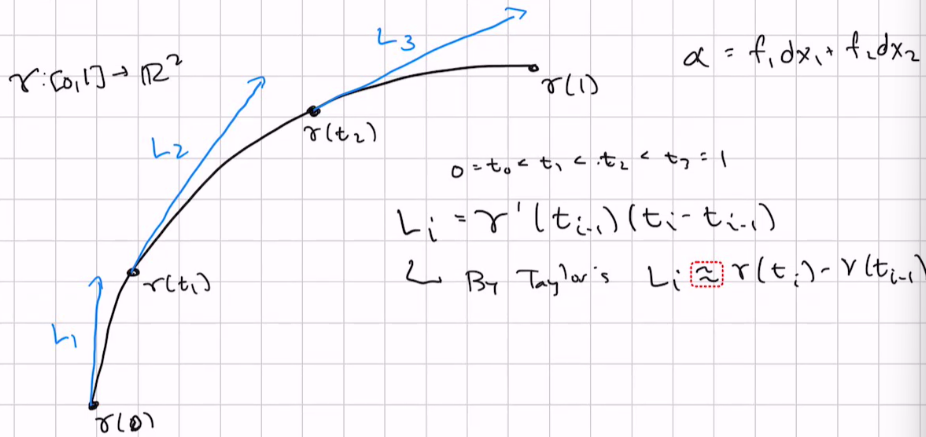
\includegraphics[width=0.5\linewidth]{Images/1-form.png}
        \caption{Visualizing $L_i$}
    \end{figure}
    Then for $k$ large,
    \begin{align*}
    \sum_{i=1}^k \alpha(L_i) &= \sum_{i=1}^k\alpha_{\gamma(t_{i-1})}\big(\gamma'(t_{i-1})(t_i - t_{i-1})\big)\\ 
    &= \sum_{i=1}^k f_1(\gamma(t_{i-1}))\gamma_1'(t_{i-1})(t_i - t_{i-1})  + f_2(\gamma(t_{i-1}))\gamma'_2(t_{i-1})(t_i - t_{i-1}) \\
    &\to \int_0^1 (f_1(\gamma(t)\gamma_1'(t) + f_2(\gamma(t))\gamma_2'(t))\,dt
    \end{align*}
    
\end{exmp}

\begin{defn}
    Let $\alpha = f_1dx_1+\dots + f_ndx_n$ be a $1-$form in $\bbR^n,$ let $\gamma: [a,b]\tp \bbR^n$ be $C^1.$ Then we define the integral of $\alpha$ over $\gamma$ to be 
    \[\int_\gamma \alpha = \int_a^b \left(f_1(\gamma(t))\gamma'_1(t) + \cdots + f_n(\gamma(t))\gamma'_n(t)\right) \, dt\]
\end{defn}
\begin{exmp}
    Let $\alpha = x^2 dx_1 + dx_2$ on $\bbR^2$ and $\gamma: [0,1]\to \bbR^2$ be $\gamma(t,t^2).$ Then 
    \[\gamma'_1(t) = 1, \quad \gamma'_2(t) = 2t.\]
    Thus, 
    \begin{align*}
        \int_\gamma \alpha &= \int_0^1 \bigg(f_1 (\gamma(t))\gamma'_1(t) + f_2(\gamma(t))\gamma'_t(t)\bigg)\,dt\\
        &= \int_0^1 \bigg(t^2 + t^2\cdot 2t\bigg)\,dt\\
        &= \int_0^1 t^2 \, dt + 2\int_0^1 t^3 \, dt\\
        &= \frac{4}{3}
    \end{align*}
\end{exmp}


\newpage
\subsection{Wednesday, Apr 30: Differential $2-$Forms}
A $2-$surface is a $C^1-$map $\gamma: I^2 \to \bbR^n.$
\begin{rem}
    Informally a \textit{$2-$form} is
    \begin{enumerate}
        \item an object which can be integrated over any $2-$surface.
        \item a rule which assigns a real number to every orientated parallelogram in $\bbR^n$ in a suitable way. 
    \end{enumerate}
Note that we specify any orientate parallelogram in $\bbR^n$ based at some $p \in \bbR^n$ by giving an ordered pair $(v,w).$ A $2-$form, $\omega,$ should satisfy:
\begin{enumerate}
    \item (Bilinear) $\omega_p(tv_1, v_2) = t\omega_p(v_1, v_2) = \omega_p(v_1, tv_2).$
    \item (Bilinear) \[\omega_p(v_1, v_2 + v_3) = \omega_p(v_1, v_2) + \omega_p(v_1, v_3)\] and 
    \[\omega_p(v_1 + v_2, v_3) = \omega_p(v_1, v_2 + v_3)\]
    \item (Asymmetric)
    \[\omega_p(v_1, v_2) = -\omega_p(v_2, v_1)\]
\end{enumerate}
Note that (c) implies that $\omega_p(v,v) = 0.$
\end{rem}
\begin{defn}
    For any $v,w \in \bbR^n,$ we denote a \textbf{basic $2-$form} by 
    \[(dx_i \wedge dx_j)(v, w) = \det\begin{pmatrix}
        v_i & w_i\\
        v_j & w_j
    \end{pmatrix}\]
\end{defn}
Intuitively, a $2-$form is the orientated area of the parallelogram's shadow on the $(i,j)$ plane!
\begin{rem}
    If $\omega_p$ satisfies (a,b,c), then $\omega_p$ can be expressed as 
    \[\omega_p = \sum_{i,j}A_{i,j}(p)(dx_i \wedge dx_j)\]
\end{rem}

\begin{defn}
    A \textbf{differential $2$-form} in $\bbR^n$ is a rule assigning a real number to each oriented parallelogram in $\bbR^n$ that can be written as 
    \[\omega = \sum_{i,j}f_{i,j}(dx_1\wedge dx_j),\] where $f_{i,j} \in C^2(\bbR^n, \bbR).$ Thus, for any $p \in \bbR^n,$ $v,w \in \bbR^n,$
    \[\omega_p(v,w) = \sum_{i,h}f_{i,j}(p)(dx_i \wedge dx_j)(v,w)\]
\end{defn}

\begin{exmp}
    Let $\omega$ be a two form in $\bbR^3.$ Then 
    \begin{align*}
    \omega &= f_{1,1}(dx_1 \wedge dx_1) + f_{1,2}(dx_1 \wedge dx_2) + f_{2,1}(dx_2 \wedge dx_1) + f_{2,2}(fx_2 \wedge dx_2)\\
    &= f_{1,2}(dx_1 \wedge dx_2) + f_{2,1}(dx_2 \wedge dx_1)\\
    &= (f_{1,2} - f_{2,1})(dx_1 \wedge dx_2)
    \end{align*}
    Thus, any $\omega$ $2-$form in $\bbR^2$ can be written as $\omega = f(dx_1 \wedge dx_2).$
\end{exmp}
\begin{exmp}
    Let $\omega$ be a two form in $\bbR^3,$ then 
    \[\omega = f_1 (dx_1 \wedge dx_2) + f_2(dx_1 \wedge dx_3) + f_3(dx_2 \wedge dx_3)\]
\end{exmp}

\begin{defn}
    Let $\gamma$ be a $C^1$ $2-$surface in $\bbR^3,$ and $\omega$ be a $2-$form in $\bbR^3.$ Then the integral of $\omega$ over $\gamma$ is 
    \begin{align*}
        \int_\gamma \omega &= \int_{I^2} \omega_{\gamma(z)} (\frac{\partial \gamma}{\partial x_1}(z), \frac{\partial \gamma}{\partial x_2}(z))\, dz \\
        &= \int_{I^2} \omega_{\gamma(z)} \left(\begin{pmatrix}
            D_1\gamma_1(z)\\
            D_1\gamma_2(z)\\
            D_1\gamma_3(z)
        \end{pmatrix}, \begin{pmatrix}
            D_2\gamma_1(z)\\
            D_2\gamma_2(z)\\
            D_2\gamma_3(z)
        \end{pmatrix}\right)\, dz \\
        &= \int_{I^2} f_1(\gamma(z))(dx_1\wedge dx_2) \left(\frac{\partial \gamma}{\partial x_1}(z), \frac{\partial \gamma}{\partial x_2}(z)\right) + f_2(\gamma(z))(dx_1\wedge dx_3) \left(\frac{\partial \gamma}{\partial x_1}(z), \frac{\partial \gamma}{\partial x_2}(z)\right) + f_3(\gamma(z))(dx_2\wedge dx_3) \left(\frac{\partial \gamma}{\partial x_1}(z), \frac{\partial \gamma}{\partial x_2}(z)\right) \, dz\\
        &= \int_{I^2}f_1(\gamma(z)) \det\begin{pmatrix}
            D_1\gamma_1(z) & D_2\gamma_1(z)\\
            D_1\gamma_2(z) & D_2\gamma_2(z)
        \end{pmatrix} + \dots \,dz
    \end{align*}
\end{defn}


\newpage
\subsection{Friday, May 2: Differential $k-$Forms}
\begin{quote}
    God grant me the serenity to accept the things I cannot change, courage to change the things I can, and wisdom to know the difference.
\end{quote}
\begin{defn}
    A $k-$surface in $\bbR^n$ is a $C^1-$map $\phi: D \to \bbR^n$ where $D$ is a $k-$cell
\end{defn}
\begin{rem}
    A $k-$form on $\bbR^n$ is a rule which assigns a real number to every orientated $k-$dimensional parallelepiped in $\bbR^n$ in a suitable way.

Note that we specify any orientated parallelepiped in $\bbR^n$ based at some $p \in \bbR^n$ by giving an ordered list $(v_1, \dots, v_k) \in T_p(\bbR^n)$ A $k-$form, $\omega,$ should satisfy:
\begin{enumerate}
    \item ($k-$tensor) \[\omega_p(v_1, \dots, tv_i, \dots, v_k) = t\omega_p(v_1, \dots, v_k)\]
    \item ($k-$tensor) \[\omega_p(v_1, \dots, v_i + w, \dots, v_k) = \omega_p(v_1, \dots, v_k) + \omega_p(v_1, \dots, w, \dots, v_k)\]
    \item (Asymmetric)
    \[\omega_p(v_1, \dots, v_i, \dots, v_j\dots, v_k) = -\omega_p(v_1, \dots, v_j, \dots, v_i,\dots, v_k)\]
\end{enumerate}
\end{rem}

\begin{defn}
    A \textbf{multi-index} of length $k$ in $\bbR^n$ is a list $I = (i_1, \dots, i_k)$ such that $i_j \in [1,n] \cap \bbN.$ 
\end{defn}

\begin{defn}
Let $I = (i_1, \dots, i_k)$ be a multi-index in $\bbR^n.$ 
    For any $v,w \in \bbR^n,$ we denote a \textbf{basic $k-$form} by 
    \[dx_I(v^1, \dots, v^k) = (dx_{i_1}\wedge \cdots \wedge dx_{i_k})(v^1, \dots, v^k) = \det \begin{pmatrix}
        v^1_{i_1} & v^2_{i_1} & \cdots & v^k_{i_1}\\
        v^1_{i_2} & v^2_{i_2} & \cdots & v^k_{i_2}\\
        \vdots &\vdots & \ddots &\vdots\\
        v^1_{i_k} & v^2_{i_k} & \cdots & v^k_{i_k}
    \end{pmatrix}\]
\end{defn}
\begin{rem}
    \begin{enumerate}
        \item If $I$ contains a repeated index, then $dx_I(v^1, \dots, v^k) = 0$ since the columns are not linearly independent.
        \item If $J$ is attained by swapping a single pair of indices in $I$, then 
        \[dx_I(v^1, \dots, v^k) = -dx_J (v^1, \dots, v^k)\]
    \end{enumerate}
\end{rem}

\begin{defn}
    A \textbf{differential $k-$form} in $\bbR^n$ is a rule assigning a real number to each oriented parallelepiped in $\bbR^n$ that can be written as 
    \[\omega = \sum_{I}f_I dx_I,\] where the sum is taken over all the multi-index $I$ of length $k$ in $\bbR^n$ and each $f_I: \bbR^n \to \bbR$ is $C^2.$  Thus, if $p \in \bbR^n,$ $v_1, \dots, v_k \in \bbR^n,$ then 
\[\omega_p(v_1, \dots, v_k) = \sum_{I} f_I(p)dx_I(v_1, \dots, v_k).\]
\end{defn}


\begin{defn}
    Let $\phi: D\to \bbR^n$ be a $k-$surface in $\bbR^n,$ and let $\omega$ be a $k-$form. Then the \textbf{integral} of $\omega$ over $\phi$ is 
    \begin{align*}
        \int_\phi \omega &= \int_D \omega_{\phi(z)} \begin{pmatrix}
            \frac{\partial \phi}{\partial u_1}( u)& \cdots& \frac{\partial \phi}{\partial u_k}( u)
        \end{pmatrix} \, du\\
        &= \int_D \sum_{I}f_I(\phi(u))dx_I\begin{pmatrix}
            \frac{\partial \phi}{\partial u_1}( u)& \cdots& \frac{\partial \phi}{\partial u_k}( u)
        \end{pmatrix} \, du\\
        &= \int_D \sum_{I} f_I(\phi(u)) J(\phi(u)) \, du
    \end{align*}
\end{defn}

\begin{exmp}
    Let $\omega = x dy \wedge dz - y dx \wedge dz + zdx \wedge dy$ be a $2-$form in $\bbR^3.$ Define the $3-$surface to be $\phi:[0,3] \times [0,2\pi] \to \bbR^3$ such that $\phi(r,\theta) = (r\cos \theta, r\sin \theta, 5)$ to be a disk of radius $r$ sitting at $z = 5.$ Let $I_1 = \{2,3\},$ $I_2 = \{1,3\}$ and $I_3 = \{1,2\}.$ Then 
    \[f_{I_1}(x,y,z) = x, \quad f_{I_2}(x,y,z) = -y, \quad f_{I_3}(x,y,z) = z.\] Then 
    \[\frac{\partial \phi}{\partial r} = \begin{pmatrix}
        \cos\theta\\
        \sin \theta\\
        0
    \end{pmatrix}\qquad \frac{\partial \phi}{\partial \theta} = \begin{pmatrix}
        -r\sin \theta\\
        r\cos \theta\\
        0
    \end{pmatrix}\] Then 
    \begin{align*}
        \int_\phi \omega &= \int_D f_{I_1}\phi(r,\theta)(dy \wedge dz)(\frac{\partial \phi}{\partial r}, \frac{\partial \phi}{\partial \theta}) + \dots \,du\\
        &= \int_D r\cos\theta\cdot 0 + (-r\sin \theta)\cdot 0+ 5r\, du\\
        &= \int_0^{3}\left(\int_0^{2\pi} 5r d\theta\right) dr\\
        &= 45 \pi
    \end{align*}
\end{exmp}


\newpage
\subsection{Monday, May 5: The Wedge Product}

\begin{defn}
    Suppose $I = (i_1, \dots, i_k)$ is a multi-index such that $i_1 < i_2< \cdots < i_k.$ We call $I$ an \textbf{increasing multi-index} and say that 
    \[dx_I =dx_{i_1} \wedge \cdots dx_{i_k}\] is a \textbf{basic $k-$form in $\bbR^n$}
\end{defn}

\begin{rem}
    The basic $k-$forms form a basis for the $k-$forms. That is, if $\omega$ is a $k-$form in $\bbR^n,$ then 
    \[\omega = \sum_I b_I dx_I.\] We note that the space of $k-$forms in $\bbR^n$ is a vector space and denote it by $\Delta^k(\bbR^n).$ The space has dimension $\binom{n}{k}.$ 
\end{rem}
\begin{exmp}
    Consider the $k-$form $dx_1 \wedge dx_2 \wedge dx_4 \wedge dx_3.$ Then 
    \[\omega = -dx_1 \wedge dx_2 \wedge dx_3 \wedge dx_4\]
\end{exmp}
\begin{defn}
    For any $\omega = \sum_I a_I dx_I,$ we can convert each $I$ into an increasing multi-index $J$ such that $\omega = \sum_J b_J dx_J.$ We call this the \textbf{standard presentation of $J$}.
\end{defn}
\begin{defn}
    Suppose $I = (i_1, \dots, i_p)$ and $J = (j_1, \dots, j_q)$ are increasing multindex. Then the \textbf{wedge product} of the corresponding forms is the $(p + q)$ form equal to 
    \[dx_I \wedge dx_J := dx_{i_1} \wedge dx_{i_2} \wedge \dots \wedge dx_{i_p} \wedge dx_{j_1} \wedge \cdots \wedge dx_{jq}.\] 
\end{defn}
\begin{rem}
    If $I$ and $J$ have no element in common (if they have one in common the wedge product is clearly $0$), we denote the increasing $(p+q)-$index obtained by arranging the elements of $I \cup J$ in increasing order by $[I,J].$ Thus, 
    \[dx_I \wedge dx_J = (-1)^\alpha dx_{[I,J]},\] where $\alpha$ is the number of swaps needed to arrange the union in increasing order.
\end{rem}

\begin{exmp}
    Suppose $\omega \in \Delta^p(\bbR^n)$ and $\lambda \in \Delta^q(\bbR^n).$ Then 
    \[\omega = \sum_I b_I dx_I, \quad \lambda = \sum_J c_J dx_J\]  and the wedge product is the $(p+q)-$form in $\bbR^n$ such that 
    \[\omega \wedge \lambda = \sum_{I,J}b_I c_J(x_I \wedge dx_J)\]
\end{exmp}

\begin{rem}
    Suppose $\omega_1, \omega_2, \lambda$ are all forms in $\bbR^n,$ then
    \begin{enumerate}
        \item (Distribution)
        \[(\omega_1 + \omega_2)\wedge \lambda = \omega_1 \wedge \lambda + \omega_2 \wedge \lambda\]
        \item (Distribution)
        \[\omega \wedge (\lambda_1 + \lambda_2) = \omega \wedge \lambda_1 + \omega \wedge \lambda_2\]
        \[(\omega \wedge \lambda) \wedge \sigma = \omega \wedge (\lambda \wedge \sigma) \]
    \end{enumerate}
\end{rem}
\begin{defn}
    A \textbf{$0$-form} in $\bbR^n$ is a $C^1(\bbR^n)$ function. 
\end{defn}
\begin{rem}
    The wedge product of a $0$ form with some $\omega \in \Delta^k(\bbR^n)$ is 
    \[f\omega:=\omega \wedge f = f\wedge \omega =:\omega f =  \sum_I fb_I dx_I\]
\end{rem}

\begin{rem}
    Informally, the differential operator assigns a $(k+1)-$form $d\omega$ to each $\omega \in \Delta^k(\bbR^n).$ 

    Suppose $f: E \to \bbR$ is a $0-$form where $f\in \Delta^0(\bbR^n).$ Then 
    \[df = D_1fdx_1 + \dots + D_nfdx_n.\]

    Suppose $\omega \in \Delta^k(\bbR^n)$ such that $\omega = \sum_I b_I dx_I.$ Then 
    \[d\omega = \sum_I (db_I)\wedge dx_I\]
\end{rem}
\begin{exmp}
    Let $\omega = xz\, dx + y^2 dz \in \Delta^2(\bbR^3).$ Then 
    \[d\omega = (z\,dx\wedge dx + 0 + \, x \,dz \wedge dx) + (0 + 2y\, dy \wedge dz + 0) = -x \,dx \wedge dz + 2y \, dy \wedge dz.\] Moreover, it can be seen that
    \[d(d\omega) = 0\]
\end{exmp}
\begin{exmp}
    Let $\pi_i: \bbR^n \to \bbR$ be the projection map of the $i^$th component. Then 
    \[d\pi_i = D_1\pi_1dx_1 + \cdots  + D_n\pi_n dx_n = dx_i.\]
\end{exmp}

\newpage
\subsection{Wednesday, May 7: Properties of the Exterior Derivative}
\begin{thm}
\begin{enumerate}
    \item (Graded Product Rule) Let $\omega \in \Delta^k(\bbR^n)$ and let $\lambda \in \Delta^m(\bbR^m)$ both of class $C^1.$ Then 
    \[d(\omega \wedge \lambda)=d\omega \wedge \lambda + (-1)^k (\omega \wedge d\lambda)\]
    \item Let $\omega \in \Delta^k(\bbR^n)$ of class $C^2,$ then $d(d\omega) = 0.$
\end{enumerate}
\end{thm}
\begin{proof}
    (a) By the distributive properties of the exterior derivative, it is enough to show this for $\omega = f dx_I$ and $\lambda = dx_J,$ where $f,g \in C^1.$ Then recall that $\omega \wedge \lambda = fg\, dx_I \wedge dx_J.$ Recall as well that $d(fg) = g\,df + f\, dg$ 
    
    If $I$ and $J$ have any common indices, then the result trivially holds. Thus, take $I$ disjoint from $J.$ Computing, noting the fifth equality comes from an identity in the homework,
    \begin{align*}
        d(\omega \wedge \lambda) &= d\left(fg \, dx_I \wedge dx_J\right)\\
        &= (-1)^\alpha d(fg \, dx_{[I,J]})\\
        &= (-1)^\alpha \left(f\,dg + g\,df\right)\wedge dx_{[I,J]}\\
        &= (f\,dg + g\, df)\wedge dx_I\wedge dx_J\\
        &= (-1)^kf \wedge dx_I \wedge dg \wedge dx_J + df\wedge dx_I \wedge g\wedge \,dx_J\\
        &= (-1)^kf  dx_I \wedge dg \wedge dx_J + df\wedge dx_I \wedge g \,dx_J\\
        &= (-1)^k (\omega d\lambda) + (d\omega \wedge \lambda)
    \end{align*}

    (b) We note that $d(d x_I) = 0$ since  by (a) we have $d(1\cdot dx_I) = d(1)\wedge dx_I = 0.$ Thus, let $f\in C^2(\bbR^n).$ We have that \[d^2(f) = d\left( \sum_{i=1}^n (D_i(f))dx_i\right) = d\left(D_1(f)dx_1 + \dots + D_n(f)dx_n\right)= \sum_{i=1}^n \left(\sum_{j=1}^n D_{ij}(f)dx_j\right) \wedge dx_i = 0.\] Thus, we see that by part (a), 
    \[d(f \wedge dx_I) = df \wedge dx_I + (-1) fd(dx_I) = 0\]
\end{proof}

\begin{defn}
    We say that $\omega \in \Delta^k(\bbR^n)$ is \textbf{closed} if $d\omega = 0.$ We say that $\omega$ is \textbf{exact} if there exists some $\alpha\in \Delta^{k-1}(\bbR^n)$ such that $d\alpha = \omega$
\end{defn}
\begin{rem}
Suppose $\omega \in \Delta^k(\bbR^n)$
    \begin{enumerate}
        \item Since $d(d(\omega)) = 0,$ then $d\omega$ is an exact form. Thus, every exact form is closed. 
        \item Not every closed form is exact. This is shown in PSET 6 question 3.
    \end{enumerate}
\end{rem}

\newpage
\subsection{Friday, May 9:  Pullbacks}
For this class, we let $E\subset \bbR^n$ and $F\subset\bbR^m$ be open, and $T: E\to F$ be $C^1.$ Let $\omega \in \Delta^k(F),$ such that 
\[\omega = \sum_{I}f_I(y) \,dy_I\] If $T(x) = (t_1(x), \dots, t_m(x)) = (y_1, \dots, y_m) = \textbf{y},$ then 
\[dt_i = \sum_{j=1}^n(D_j t_i)\, dx_j\] is a one form on $E.$ Thus, $T$ transforms $\omega$ by pulling it back to $E.$ 
\begin{defn}
    The \textbf{pullback form} of $\omega$ is 
    \[\omega_T(x) = \sum_{I}f_I(T(x))\,dt_{I}\]
\end{defn}
\begin{exmp}
    Let $T: \bbR^n \to \bbR^n$ be the identity mapping. Let $\omega = \sum_I f_I \,dx_I$. Then $t_i(x) = x_i,$ 
    \[dt_i = D_1 x_i \,dx_1 + \dots + D_n x_i \, dx_n =   dx_i,\] and so 
    \[\omega_T(x) = \sum_I f_I(x)\, dx_I\]
\end{exmp}
\begin{exmp}
    Let $T: \bbR^2 \to \bbR^3$ such that 
    \[(x_1, x_2)\mapsto (x_2, x_1^2, x_1 + x_2) = (t_1, t_2, t_3).\] Let $\omega \in \Delta^2(\bbR^3)$ such that 
    \[\omega(y_1, y_2, y_3) = y_1\,dy_2 \wedge dy_3.\] Computing, we see that 
    \[dt_1 = dx_2, \quad dt_2 = 2x_1\,dx_1, \quad dt_3 = dx_1 + dx_2,\] and so 
    \begin{align*}
        \omega_T(x_1, x_2) &= f_{2,3}(T(x_1, x_2)) \,(dt_2 \wedge dt_3)\\
        &= f_{2,3}(x_2, x_1^2, x_1 + x_2) \,(2x_1\,dx_1) \wedge (dx_1 + dx_2)\\
        &= (2x_1x_2)\,(dx_1 \wedge dx_1 + dx_1 \wedge dx_2)\\
        &= 2x_1x_2\, dx_1 \wedge dx_2
    \end{align*}
\end{exmp}
\begin{lemma}
    Let $f\in C^1(F, \bbR).$ Then if we call $f_T = f\circ T,$ 
    \[d(f_T) = (df)_T.\]
\end{lemma}
\begin{proof}
    Follow your nose and use change of variable
    \begin{align*}
        d(f_T) &= \sum_{j=1}^n D_j f_T\,dx_j\\
        &= \sum_{j=1}^n D_j (f\circ T)dx_j\\
        &= \sum_{i=1}^m \sum_{j=1}^n (D_if_i)(T)\cdot D_jt_i\,dx_j\\
        &= \sum_{i=1}^m (D_if)(T)dt_i\\
        &= (df)_T
    \end{align*}
\end{proof}

\begin{thm}
    Let $\omega\in \Delta^k(F)$ and $\lambda\in \Delta^l(F).$ If $T: E\to F$ is $C^1,$ then 
    \begin{enumerate}
        \item if $k = l,$ $(\omega + \lambda)_T = \omega_T + \lambda_T$
        \item $(\omega\wedge\lambda)_T = \omega_T\wedge\lambda_T$
        \item $d(\omega_T) = (d\omega)_T$ if $T\in C^2(E,F)$
    \end{enumerate}
    \begin{proof}
        (i) Let $\omega = \sum_I f_I dy_I$ and $\lambda = \sum_I g_I dy_I.$ Then 
        \begin{align*}
            (\omega + \lambda)_T &= \left(\sum_I (f_I + g_I)\,dy_I\right)_T\\
            &= \sum_I (f_I + g_I)(T)\, dt_I\\
            &= \omega_T + \lambda_T
        \end{align*}
        The proof for (ii) is on PSET 7.

        (iii) Suppose $T\in C^2(E,F).$ First consider the case when 
        \[\omega = dy_{i_1} \wedge \dots \wedge dy_{i_k}, \quad \omega_T = dt_{i_1} \wedge \dots \wedge dt_{i_k}.\] We use the graded product rule to easily conclude that 
        \[d\omega =0 = d(\omega_T),\] and so $(d\omega)_T = 0.$ For the general case, use the previous lemma.
    \end{proof}
\end{thm}


\newpage
\subsection{Monday, May 12: Change of Variables}
For this class, we let $E\subset \bbR^n$ and $F\subset\bbR^m$ be open.
\begin{thm}
    If $T \in C^1(E, F),$ and $S\in C^1(F, G),$ where $G \subseteq \bbR^\ell,$ and $\omega\in \Delta^k(G).$   Then 
    \[(\omega_S)_T = \omega_{S\circ T}\]
\end{thm}
\begin{rem}
    As a remark, note that $\omega_S \in \Delta^k(G)$ and $(\omega_S)_T, \omega_{S\circ T} \in \Delta^k(E).$
\end{rem}
\begin{thm}
    Suppose $\omega\in \Delta^k(E),$ and $\phi$ is a $k-$surface in $E$ with parameter domain $D\subseteq \bbR^k.$ If $\Delta$ is the trivial $k-$surface, $\Delta: D\to \bbR^k,$ where $\Delta(u) = u,$ then 
    \[\int_\phi \omega = \int_\Delta \omega_\phi\]
\end{thm}
\begin{proof}
    It suffices to show this for the case when 
    \[\omega = f\,dx_I = f\,dx_{i_1}\wedge \dots \wedge dx_{i_k}.\] Let $\phi_i, \dots, \phi_n$ denote the components of $\phi.$ Then 
    \[\omega_\phi = \sum_{I} f_I(\phi)\,d\phi_I = f(\phi)\,d\phi_{i_1}\wedge \dots \wedge d\phi_{i_k}.\] It suffices to show that
    \begin{align}
    d\phi_{i_1}\wedge \dots \wedge d\phi_{i_k} = J (u) \,du_1\wedge \dots \wedge du_k, 
    \end{align}
     where $J(u) = \frac{\partial (x_1, \dots, x_{i_k})}{\partial (u_1, \dots, u_k)}.$ Assuming (1), 
     \begin{align*}
         \int_\Delta \omega_\phi &= \int_\Delta f(\phi)\,d\phi_{i_1}\wedge \dots \wedge d\phi_{i_k}\\
         &= \int_\Delta f(\phi) J(u) \,du_1\wedge \dots \wedge du_k\\
         &= \int_D f(\phi (u))J(u)du\\
         &= \int_\phi \omega.
     \end{align*}
     To prove (1), let $[A]$ be the $k\times k$ matrix with entries
     \[\alpha(p,q) = (D_q\phi_p)(u)\] for all $p,q = 1,\dots, k.$ Note that $\det A = J(u).$ Since 
     \[d\phi_{i_p} = \sum_{q}\alpha(p,q)\,du_{q}\] Thus, 
     \[d\phi_{i_1}\wedge \dots \wedge d\phi_{i_k} = \sum \alpha(1,q_1)\cdots \alpha(k,q_k) \,du_{q_1}\wedge \dots \wedge du_{q_k},\] where the sum ranges over all the $q_1, \dots, q_k \in \{1,\dots, k\}.$ In order to get the wedge product into standard presentation, we rearrange 
     $du_{q_1}\wedge \dots \wedge du_{q_k}$ to get 
     \[d\phi_{i_1}\wedge \dots \wedge d\phi_{i_k} = (\det A)\, du_1 \wedge \dots \wedge du_k = J(u)\,du_1 \wedge \dots \wedge du_k\]
 \end{proof}
\begin{exmp}
    Consider when $k = 2.$
\[ A = \begin{bmatrix}
     \alpha(1,1) & \alpha(1,2)\\
     \alpha(2,1) & \alpha()2,2
 \end{bmatrix}\]
 Then 
 \begin{align*}
 d\phi_{i_1}\wedge d\phi_{i_2} &= \alpha(1,1)\alpha(2,1)\, du_{1}\wedge du_{1} + \alpha(1,1)\alpha(2,2)\,du_{1}\wedge du_{2} \\
 &+ \alpha(1,2)\alpha(2,1)\,du_2 \wedge du_1 + \alpha(2,2)\alpha(1,2)\,du_2\wedge du_2\\
 &= (\alpha(1,1)\alpha(2,2) - \alpha(1,2)\alpha(2,1))\,du_1\wedge du_{2}\\
 &= \det(A)\,du_1 \wedge du_2
 \end{align*}
 
\end{exmp}

\begin{thm} (Change of Variables)
    Suppose $T\in C^1(E,F)$ and $\phi$ is a $k-$surface in $E.$ If $\omega\in \Delta^k(F),$ then 
    \[\int_{T\circ \phi} \omega = \int_\phi \omega_T\]
\end{thm}
\begin{proof}
    Let $D$ be the parameter domain of $\phi$ (and thus of $T\circ \phi$).  Let $\Delta: D \to D$ be the identity map on $D$ such that $\Delta(u) = u.$ Then by Theorem 21 and Theorem 20 and Theorem 21 again,
    \[\int_{T\circ \phi} \omega = \int_\Delta \omega_{T\circ \phi} = \int_\Delta (\omega_T)_\phi  = \int_\phi \omega_T\]
\end{proof}

\begin{defn}
    A map $f: X\to Y,$ where $X,Y$ are vector spaces, is called \textbf{affine} if $f - f(0)$ is linear.
\end{defn}
\begin{rem}
    In other words, $f$ is affine if 
    \[f(x) = f(0) + Ax,\quad A:X\to Y \text{ is linear}.\] An affine map from $\bbR^k \to \bbR^n$ is determined by $f(0)$ and its value for each $f(e_i).$
\end{rem}

\begin{defn}
    The \textbf{$k-$simplex} in $\bbR^k$ is $Q^k \subseteq \bbR^k$ such that 
    \[Q^k:= \{x = (x_1, \dots, x_k)\mid x_i \geq 0, \,\sum_{i=1}^k x_i \leq 1\}\]
\end{defn}
\begin{rem}
    The one simplex is $[0,1].$ The two-simplex is the right triangle with endpoints $(0,0), (0,1), (1,0).$ 
\end{rem}


\newpage
\subsection{Wednesday, May 14: Oriented Simplexes}
\begin{defn}
    Let $p_0, p_1, \dots, p_k \in \bbR^n.$ The \textbf{oriented affine $k-$simplex} $\sigma = [p_0, \dots, p_k]$ is the $k-$surface in $\bbR^n$ with parameter domain $Q^k$ given by the affine map 
    \[\sigma(\alpha_1\,e_1, \dots, \alpha_k \,e_k) = p_0 + \sum_{1}^k \alpha_i(p_i - p_0)\]
\end{defn}
\begin{rem}
   For all $u \in Q^k,$ we can write $\sigma(u) = p_0 + Au,$  where $A \in L(\bbR^k, \bbR^n)$ such that $Ae_i = p_i - p_0.$ 

   For intuition, $\sigma$ is a map from the endpoints of $Q^k$ to the points $p_0, \dots, p_k.$ 

   $\sigma$ is called oriented to emphasize that the order of the points $p_0, \dots, p_k$ matters. To illustrate this, consider $\overline{\sigma} = [p_{i_0}, \dots, p_{i_k}],$ where $\{i_0, \dots, i_k\}$ is a permutation of $\{0,1,\dots, k\}.$ Then 
   \[\overline{\sigma} = s(i_0, \dots, i_k)\sigma, \quad s(\vec{i_j}) = (-1)^\alpha, \alpha\text{ is min \# swaps needed to permute $i_0, \dots, i_k$ to $0, \dots, k$}\] Suppose $\overline{\sigma} = \varepsilon\sigma,$ where $\varepsilon = \pm 1.$ If $\epsilon = 1,$ we say that $\overline{\sigma}$ and $\sigma$ have the same orientation. Otherwise, we say that they have opposite orientations.
\end{rem}

\begin{defn}
    An \textbf{oriented $0$-simplex} is a point $p_0 \in \bbR^n$ with a sign attached. We write $\sigma = \pm p_0.$ If $f$ is a $0-$form, $\sigma = \varepsilon p_0,$ where $\varepsilon = \pm1 ,$ then 
    \[\int_\sigma f = \varepsilon f(p_0).\]
\end{defn}
\begin{thm}
    If $\sigma$ is an oriented $k-$simplex in $E\subseteq \bbR^n$ open and if $\overline{\sigma} = \varepsilon \sigma,$ $\varepsilon = \pm 1,$ then for all $\omega \in \Lambda^k(E)$ is given by 
    \[\int_\sigma \omega = \varepsilon \int_{\overline{\sigma}}\omega\]
\end{thm}

\begin{defn}
    An \textbf{affine $k-$chain} $\Gamma$ in an open set $E\subseteq \bbR^n$ is a collection of finitely many oriented affine $k-$simplexes in $E,$ denoted by
    \[\sigma_1, \dots, \sigma_r\]
\end{defn}
Note that $\Gamma$ may not be distinct, there might be multiples of the same simplex many times within the same chain.
\begin{defn}
    If $\Gamma$ is an affine $k-$chain is $E\subseteq \bbR^n$ and $\omega \in \Lambda^k(E),$ then 
    \[\int_\Gamma \omega = \sum_{i=1}^r \int_{\sigma_i} \omega\] 
\end{defn}
\begin{rem}
    We will often abuse notation and write formally 
    \[\Gamma = \sigma_1 + \dots+ \sigma_r = \sum_{1}^r \sigma_i.\]
\end{rem}
\begin{exmp}
    Consider 
    \[\sigma_1 = [p_0, p_1, p_2], \quad \sigma_2 = [p_1, p_0, p_2],\] where $\sigma_1 = -\sigma_2.$ 
\[    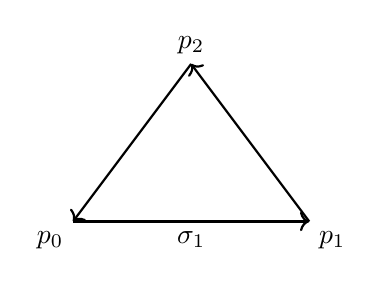
\begin{tikzpicture}
    % Points
    \coordinate (P0) at (0, 0);
    \coordinate (P1) at (3, 0);
    \coordinate (P2) at (1.5, 2);

    % Edges and Labels
    \draw[thick, ->] (P0) -- (P1) node[midway, below] {$\sigma_1$};
    \draw[thick, ->] (P1) -- (P2);
    \draw[thick, ->] (P2) -- (P0);

    % Points Labels
    \node[below left] at (P0) {$p_0$};
    \node[below right] at (P1) {$p_1$};
    \node[above] at (P2) {$p_2$};

\end{tikzpicture}\]



% Simplex Sigma_2 (Reversed Orientation)
\[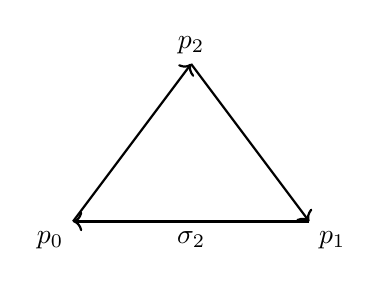
\begin{tikzpicture}
    % Points
    \coordinate (P0) at (0, 0);
    \coordinate (P1) at (3, 0);
    \coordinate (P2) at (1.5, 2);

    % Edges and Labels
    \draw[thick, ->] (P1) -- (P0) node[midway, below] {$\sigma_2$};
    \draw[thick, ->] (P0) -- (P2);
    \draw[thick, ->] (P2) -- (P1);

    % Points Labels
    \node[below left] at (P0) {$p_0$};
    \node[below right] at (P1) {$p_1$};
    \node[above] at (P2) {$p_2$};

\end{tikzpicture}\]

If $\Gamma = \sigma_1 + \sigma_2,$ then if $\omega \in \Lambda^2(E),$ we have that by Theorem 23,
\[\int_\Gamma \omega = \int_{\sigma_1}\omega + \int_{\sigma_2}\omega = \int_{\sigma_1}\omega - \int_{\sigma_1}\omega = 0.\] Thus, we abuse notation again and write 
\[\Gamma = 0\]

Moreover, we note that the boundary of $\sigma_1$ is simply three lines (a triangle), making 
\[\partial \sigma_1 = \sigma'_1 + \sigma_2' + \sigma_3',\] where $\sigma_i'$ are all oriented affine $1-$simplexes.
\end{exmp}


\begin{defn}
    For $k \geq 1,$ the boundary of an orientated affine $k-$simplex  $\sigma = [p_0, \dots, p_k]$ is the affine $(k-1)$ chain
    \[\partial \sigma = \sum_{j=0}^k (-1)^k [p_0, \dots, p_{j-1}, p_{j+1}, p_k]\]
\end{defn}
\begin{exmp}
    Consider $\sigma = [p_0, p_1, p_2]$ to be the filled in triangle. By definition
    \[\partial \sigma = [p_1, p_2] - [p_0, p_2] + [p_0, p_1] = [p_1, p_2] + [p_2, p_0] + [p_0, p_1]\]
\end{exmp}
\begin{exmp}
    Consider the tetrahedron $\sigma = [p_0, \dots, p_3].$ Intuitively, the boundary of the tetrahedron are the faces of the triangles. Formally, 
    \[\partial \sigma = [p_1, p_2, p_3] - [p_0, p_2, p_3] + [p_0, p_1, p_2] - [p_0, p_1, p_2]\]
\end{exmp}


\newpage
\subsection{Friday, May 16: Introducing Stokes Theorem}
\begin{defn}
    Let $T \in C^2(E, F).$ Let $\sigma$ be an oriented affine $k-$simplex in $E.$ The map $\phi: T\circ \sigma$ is a $k=$surface in $F.$ We call $\phi$ an \textbf{oriented $k-$simplex.}
\end{defn}
\begin{defn}
    A finite collection $\Psi$ of oriented $k-$simplex, $\{\phi_1, \dots, \phi_r\}$ is called a \textbf{$k-$chain} of class $C^2$ in $F.$ 
\end{defn}
Formally, we denote $\Psi = \sum \phi_i$
\begin{defn}
    If $\omega \in \Lambda^k(F),$ we define 
    \[\int_\Psi \omega = \sum_{i=1}^r \int_{\phi_i}\omega\]
\end{defn}

If $\Gamma = \sum \sigma_i$ and $\phi_i = T \circ \sigma_i$, we formally write $\Psi = T \circ \Gamma.$

\begin{defn}
    The \textbf{boundary of an oriented $k-$simplex} $\phi = T\circ \sigma$ is the $k-1$ chain defined by
    \[\partial \phi = T\circ \partial \sigma.\]
\end{defn}
Note that if $\phi \in C^2(E,F),$ then so is $\partial \phi.$ 
\begin{defn}
    The {boundary of a $k-$chain }$\Psi = \sum \phi_i$ is the $k-1$chain denoted 
    \[\partial T = \sum \partial \phi_i\]
\end{defn}

\begin{thm}
    (Stokes) If $\Psi \in C^2(E,F)$ is a $k-$chain, $\omega \in \Lambda^{k-1}(F)$ of class $C^1,$ then 
    \[\int_\Psi d\omega = \int_{\partial \Psi}\omega\]
\end{thm}
The proof is deferred till next class.
\begin{rem}
    A few consequences of the FTC:
    \begin{enumerate}
        \item (FTC)
        
        When $k = m = 1,$ then $\omega = f \in C^1(E,F).$ Since $m = 1,$ then $F = \subseteq \bbR.$ It suffices the case when 
        \[\Psi = \sigma = [a,b].\] Thus, the boundary is a $0-$chain of oriented points:
        \[\partial \sigma = [b] - [a].\] Thus, by definition
        \[\int_{\partial \sigma} f = \int_{[b]} f - \int_{[a]} f = f(b) - f(a).\] Thus, 
        \[f(b) - f(a) = \int_{\Psi} d\omega = \int_{\sigma} df = \int_a^b df(x)\,dx\]
    \item (Green's Thm) is the case when $k = m = 2.$ To see this, consider a smooth vector field $F: \bbR^2 \to \bbR^2.$ We can write $F = F_1 + F_2,$ where $F_1$ and $F_2$ are the $x$ and $y$ components of $F.$ Green's Theorem states that if $D$ is a surface in $\bbR^2$ bounded by a curve $C,$ then 
    \[\int_C F_1 \,dx + F_2\,dy = -\int_D \left(\frac{d F_2}{d x}- \frac{dF_1}{dy}\right) \,dx\,dy.\]
Let 
\[\omega = F_1\,dx++ F_2\,dy \in \Lambda^1(\bbR^2).\] Then Stokes' theorem states that 
\[\int_C F_1 dx + F_2dy= \int_{\partial D} \omega = \int_D d\omega = \int_D \frac{\partial F_1}{\partial y}\,dy \wedge dx +  \frac{\partial F_2}{\partial x}\,dx \wedge dy= \int_D \left(\frac{\partial F_2}{\partial x} - \frac{\partial F_1}{\partial y}\right)\,dxdy\]
    
    \item (Divergence) is the case when $k = m = 3.$
Consider a smooth vector field $F: \bbR^3 \to \bbR^3,$ writing $F = F_1 + F_2 + F_3.$ Let $\omega^2_F = F_1 \,dx\wedge dy + F_2 \,dz\wedge dx + F_3\,dy\wedge dz.$ We have shown that $d\omega_F^2 = (\nabla \cdot F) dx\wedge dy \wedge dz = (\div F)dV.$ Thus, we have by Stokes' Theorem that 
\[\int_{\Phi}(\div F)dV = \int_\Phi d\omega_F^2 = \int_{\partial \Phi}\omega_F^2 = \int_{\partial\Phi} F\cdot n\]
    \item (OG Stokes) is the case when $k = 2$ and $m =3.$ 
    \end{enumerate}
\end{rem}

\begin{thm}
    (Baby Stokes) Let $E\subset \bbR^k$ containing $Q^k.$ Let $\sigma = [0, e_1, \dots, e_k].$ Let $\lambda \in \Lambda^{k-1}(E)$ of class $C^1.$ Then 
    \[\int_{\sigma} d\lambda = \int_{\partial \sigma} \lambda.\]
\end{thm}
The proof is again differed to next class. 

\begin{prop}
    To prove Stokes' Theorem, it suffices to prove Baby Stokes.
\end{prop}
\begin{proof}
    It suffices to prove stokes with $\Psi = \phi$ by the linearity of addition. Moreover, it suffices to prove Stokes when $\Psi = \phi$ and $\phi = \sigma,$ where $\sigma$ is an affine $k-$simplex. To show this, we suppose $\phi = T\sigma.$ Then using Theorem 22 (Change of Var)
    \[\int_\Psi d\omega = \int_{T\sigma} d\omega = \int_\sigma (d\omega)_T = \int_\sigma d(\omega_T)\] Supposing Baby stokes, 
    \[\int_\sigma d(\omega_T) = \int_{\partial \sigma} \omega_T = \int_{T\circ \partial \sigma} \omega = \int_{\partial \psi}\omega.\] It remains to show that is suffices to show that Stokes holds when $\sigma = [0, e_1, \dots, e_k].$ Let $\Psi = T \sigma,$ where $T$ is affine. Then 
    \[\int_{\Psi}d\omega = \int_{T \circ \sigma} d\omega = \int_\sigma d(\omega_T) = \int_{\partial \sigma} \omega_T = \int_{T\circ \partial \sigma}\omega = \int_{\partial \Psi}\omega\]
\end{proof}
\newpage
\subsection{Monday, May 19: Stokes Theorem}
We prove Baby Stokes (Theorem 25)
\begin{proof}
    If $k =1 ,$ the conclusion follows by FTC. Fix $r$ such that $1\leq r \leq k,$ and let $f \in C^1(E).$ It suffices to prove the conclusion when 
    \[\lambda = f dx_1 \wedge \dots dx_{r-1}\wedge dx_{r+1}\wedge \cdots \wedge dx_k.\] By definition, 
    \[\partial \sigma = [e_1, \dots, e_k] + \sum_{j=1}^\infty (-1)^i \tau_i,\] where 
    \[\tau_i = [0,e_1, \dots, e_{i-1}, e_{i+1}, \dots, e_k].\] For convenience, we let 
    \[\tau_0:= [e_r, e_1, \dots, e_{r-1}, e_{r +1}, \dots, e_k]  = (-1)^{r-1}[e_1, \dots, e_k].\] Let $u\in \bbQ^{k-1}$ and let $x = (x_1, \dots, x_k) = \tau_0(u).$ Then the $j$th component of $x$ is given by
    \[x_j  = \begin{cases}
        u_j \qquad \qquad \qquad \quad \qquad  1\leq j \leq r-1\\
        1-(u_1 + \cdots + u_k) \qquad j = r\\
        u_{j-1}\qquad \quad \qquad \qquad r + 1 \leq j \leq k
    \end{cases}\]

    Let $x = \tau_i(u),$ where $i \neq 0.$ Then 
        \[x_j  = \begin{cases}
        u_j \qquad  1\leq j \leq i-1\\
        0 \qquad j = i\\
        u_{j-1} \quad i + 1 \leq j \leq k
    \end{cases}\]

    Let $J_{i}$ be the Jacobian of the map $u_1, \dots, u_{k-1}\mapsto (x_1, \dots, x_{r-1}, x_{r + 1}, \dots, x_k)$ induced by $\tau_i.$ Then if $i = 0,$ $J_0 = 1$ since the map is the identity map. If $i = r,$ then $J_r = 1.$ For any other $i,$ $J_i = 0.$ Then by definition, 
    \begin{align*}
    \int_{\partial \sigma}\lambda &= (-1)^{r-1}\int_{\tau_0}\lambda + (-1)^r \int_{\tau_r}\lambda\\
    & =(-1)^{r-1}\left[\int_{\tau_0}\lambda - \int_{\tau_r}\lambda \right]\\
    &=(-1)^{r-1}\left[\int_{Q^{k-1}}f(\tau_0(u))\,du - \int_{Q^{k-1}}f(\tau_r(u))\,du\right]\\ 
    &= (-1)^{r-1}\int_{Q^{k-1}} \left[f(\tau_0(u)) - f(\tau_r(u))\right]du
    \end{align*}
    On the other hand, 
    \begin{align*}
      d\lambda &= \left(\sum_i^k D_if \,dx_k\right)\wedge dx_1 \wedge \cdots\wedge dx_{r-1}\wedge dx_{r+1}\wedge \cdots \wedge dx_k\\ &= D_r f\,dx_r \wedge dx_1 \wedge \cdots\wedge dx_{r-1}\wedge dx_{r+1}\wedge \cdots \wedge dx_k  \\
      &= (-1)^{r-1} D_r f\, dx_1 \wedge \cdots \wedge dx_k\\
    \end{align*}
    Then by definition,
    \begin{align*}
        \int_\sigma d\lambda &= (-1)^{r-1}\int_{Q^k}D_r f(x)\,dx\\
        &= (-1)^{r-1} \int_{Q^{k-1}}\left(\int_0^{1-x_r - x_{r-1} + \cdots x_1} D_rf(x)\,dx_r\right)dx_1 dx_1\cdots dx_{r-1}dx_{r+1}\cdots dx_k\\
        &= (-1)^{r-1}\int_{Q^{k-1}}f(1- (\sum_{1}^r x_i)) - f(0)\,du\\
        &= (-1)^{r-1}\int_{Q^{k-1}}f(\tau_0(u)) - f(\tau_r(u))\,du
    \end{align*}
\end{proof}
By proposition 3, we have proved Stokes theorem.

\newpage
\subsection{Wednesday, May 21: Baire Category}
\begin{defn}
    Let $X$ be a metric space with metric $d.$ Let $E\subseteq X.$
    \begin{enumerate}
        \item The \textbf{interior} of $E$ is 
        \[E^\circ  = \bigcup G_n,\] where $G_n \subseteq E$ are open.
        \item The \textbf{closure} of $E$ is 
        \[\overline{E} = \bigcap F_n,\] where $F_n \supset E$ are closed.
        \item We say that $E$ is \textbf{dense} in $X$ if 
        \[\overline{E}= X.\]
        \item We say that $E$ is \textbf{nowhere dense} if 
        \[(\overline{E})^\circ  = \emptyset\]
        \item We say that $E$ is of \textbf{first category} or \textbf{meager} if 
        \[E = \bigcup E_n,\] where $E_n$ are nowhere dense sets (e.g, the rationals)
        \item If $E$ is not of first category, then $E$ is \textbf{second category}.
        \item If $E^c$ is of first category, then $E$ is said to be a \textbf{residual} or \textbf{generic} set.
    \end{enumerate}
\end{defn}

\begin{thm}
    (Baire Category) If $X$ is a complete metric, then $X$ is of second category. That is, if $X = \bigcup F_n,$ where each $F_n$ is closed, then at least one of the $F_n$ is not nowhere dense.
\end{thm}

\begin{proof}
    Suppose $X$ is not of second category. Then $X  = \bigcup F_n,$ where $F_n$ are nowhere dense. Without loss of generality, take $F_n$ to be closed. We will show that there exists some $x\in X$ such that $x\notin \bigcup F_n.$ Since $F_1$ closed and nowhere dense, then $F_1 \neq X$ and there is some ${r_1}>0$ and $x_1 \in X\sm F_1$ such that $\overline{B_{r_1}(x_1)} \subseteq F_1^c.$ Since $F_2$ is  nowhere dense, then $B_{r_1}(x_1)\not\subseteq F_2.$ Let $x_2 \in B_{r_1}(x_1) \sm F_2.$ There is some $0<r_2< \frac{r_1}{2}$ such that $\overline{B_{r_2}(x_2)}\subseteq B_{r_1}(x_1)$ and $\overline{B_{r_2}(x_2)}\subseteq F_2^c.$ We obtain a sequence of balls with \[B_1\supset B_2 \supset \cdots \] and $r_1, r_2,\dots,$ such that $r_n \to 0$ and  $F_n \cap \overline{B}_n= 0.$ The sequence $\{x_n\}$ is clearly Cauchy and thus converges to some $x_\infty \in X.$ But since $x_\infty \in \bigcap B_n,$ $x_\infty \notin F_n$ for all $n \in \bbN.$ Thus, $x_\infty \notin \bigcup F_n,$ a contradiction! Hence, $X$ is of second category.  
\end{proof}
\begin{cor}
    If $X$ is complete, then a residual set of $X$ is dense. 
\end{cor}
\begin{proof}
    Let $E$ be residual, and suppose $E$ is not dense. Thus, there exists some $\overline{E} \neq X.$ Thus, there exists some $r>0$ such that $B = B_r(x) \subset E^c$ where $x\in E^c.$ We know that $E^c$ is of first category. I.e, 
    \[E^c = \bigcup_{n=1}^\infty F_n,\] where $F_n$ are nowhere dense. Thus, 
    \[\overline{B} = \bigcup_{1}^\infty (F_n \cap \overline{B}).\] But $\overline{B}$ is a complete metric space, contradiction BCT.
\end{proof}

For the following, we let $X = C([0,1], \bbR)$ be equipped with the $\sup$ metric, i.e.
\[d(f,g) = \|f-g\| = \sup_{x\in [0,1]}|f(x) - g(x)|.\]
We have shown $(X,d)$ to be complete. 

\begin{thm}
    The set of functions $f \in X$ that are nowhere differentiable is residual.
\end{thm}
\begin{proof}
    Let $D= \{f \in X \mid f'(x) \text{ exists for some }x\in [0,1]\}.$ It suffices to show that $D$ is of first category. That is, it suffices to show that 
    \[D = \bigcup_{n=1}^\infty D_n,\] where the $D_n$ are nowhere dense. Consider defining 
    \[D_n = \{f\in X \mid \exists x^* \in [0,1] : |f(x) - f(x^*)| \leq n|x-x^*|\forall x\in [0,1] \}.\] We know that 
    \[D \subseteq \bigcup_{n=1}^\infty D_n\]
\begin{lemma}
    $D_n$ is closed.
\end{lemma}
\begin{proof}
    Let $(f_k) \in D_n$ such that $f_k \to f.$ It suffices to show that $f\in D_n.$ Since $f_k \in D_n,$ then for each $f_k,$ there exists some $x^*_k \in [0,1]$ such that $|f_k(x) - f_k(x^*_k)| \leq n|x - x^*_k|$ for all $x\in [0,1].$ Consider that $(x^*_k)$ is a sequence of real numbers, and thus has a subsequence converging to some $x^*$.
    Using the triangle inequality, we have that for large enough $k_j,$ 
    \begin{align*}
|f(x) - f(x^*)| &\leq |f(x) - f_{k_j}(x)| + |f_{k_j}(x) - f_{k_j}(x^*)| + |f_{k_j}(x^*) - f(x^*)|    \\
&\leq \|f - f_{k_j}\| + |f_{k_j}(x) - f_{k_j}(x^*)| + \|f- f_{k_j}\|\\
&\leq \epsilon + |f_{k_j}(x) - f_{k_j}(x^*)|\\
&\leq \epsilon + |f_{k_j}(x) - f_{k_j}(x^*_{k_j})| + |f_{k_j}(x_{k_j}^*) - f_{k_j}(x^*)|\\
&\leq \epsilon + n|x - x_{k_j}^*| + n|x_{k_j}^* - x^*|\\
&\leq \epsilon + n|x - x_{k_j}^*| + \epsilon\\
&\leq 2\epsilon + n(|x-x^*| + |x^* - x_{k_j}^*|)\\
&\leq 3\epsilon + n|x - x^*|
    \end{align*}
    Taking $\epsilon \to 0,$ we see that $f\in D_n.$ 
\end{proof}
\begin{lemma}
    $D_n$ is nowhere differentiable.
\end{lemma}
\begin{proof}
    Let $\mathcal{P}\subseteq X$ be the set of piecewise linear functions in $C([0,1]).$ Let $\mathcal{P}_m\subseteq \mathcal{P}$ be the piecewise continuous functions in $\mathcal{P}$ such that the if $\beta$ is a slope of any line segment in $f \in \mathcal{P}_m$, then $|\beta|\geq M.$ We claim that $\mathcal{P}_M$ is dense in $X$ for all $M \geq 0.$
\end{proof}

\end{proof}

\end{document}